%%
% Copyright (c) 2017 - 2020, Pascal Wagler;
% Copyright (c) 2014 - 2020, John MacFarlane
%
% All rights reserved.
%
% Redistribution and use in source and binary forms, with or without
% modification, are permitted provided that the following conditions
% are met:
%
% - Redistributions of source code must retain the above copyright
% notice, this list of conditions and the following disclaimer.
%
% - Redistributions in binary form must reproduce the above copyright
% notice, this list of conditions and the following disclaimer in the
% documentation and/or other materials provided with the distribution.
%
% - Neither the name of John MacFarlane nor the names of other
% contributors may be used to endorse or promote products derived
% from this software without specific prior written permission.
%
% THIS SOFTWARE IS PROVIDED BY THE COPYRIGHT HOLDERS AND CONTRIBUTORS
% "AS IS" AND ANY EXPRESS OR IMPLIED WARRANTIES, INCLUDING, BUT NOT
% LIMITED TO, THE IMPLIED WARRANTIES OF MERCHANTABILITY AND FITNESS
% FOR A PARTICULAR PURPOSE ARE DISCLAIMED. IN NO EVENT SHALL THE
% COPYRIGHT OWNER OR CONTRIBUTORS BE LIABLE FOR ANY DIRECT, INDIRECT,
% INCIDENTAL, SPECIAL, EXEMPLARY, OR CONSEQUENTIAL DAMAGES (INCLUDING,
% BUT NOT LIMITED TO, PROCUREMENT OF SUBSTITUTE GOODS OR SERVICES;
% LOSS OF USE, DATA, OR PROFITS; OR BUSINESS INTERRUPTION) HOWEVER
% CAUSED AND ON ANY THEORY OF LIABILITY, WHETHER IN CONTRACT, STRICT
% LIABILITY, OR TORT (INCLUDING NEGLIGENCE OR OTHERWISE) ARISING IN
% ANY WAY OUT OF THE USE OF THIS SOFTWARE, EVEN IF ADVISED OF THE
% POSSIBILITY OF SUCH DAMAGE.
%%

%%
% This is the Eisvogel pandoc LaTeX template.
%
% For usage information and examples visit the official GitHub page:
% https://github.com/Wandmalfarbe/pandoc-latex-template
%%

% Options for packages loaded elsewhere
\PassOptionsToPackage{unicode}{hyperref}
\PassOptionsToPackage{hyphens}{url}
\PassOptionsToPackage{dvipsnames,svgnames*,x11names*,table}{xcolor}
%
\documentclass[
  14pt
  american,
  paper=a4,
  ,captions=tableheading
]{scrreprt}
\usepackage{amsmath,amssymb}
\usepackage{lmodern}
\usepackage{setspace}
\setstretch{1.2}
\usepackage{amsmath}
\usepackage{ifxetex,ifluatex}
\ifnum 0\ifxetex 1\fi\ifluatex 1\fi=0 % if pdftex
  \usepackage[T1]{fontenc}
  \usepackage[utf8]{inputenc}
  \usepackage{textcomp} % provide euro and other symbols
  \usepackage{amssymb}
\else % if luatex or xetex
  \usepackage{unicode-math}
  \defaultfontfeatures{Scale=MatchLowercase}
  \defaultfontfeatures[\rmfamily]{Ligatures=TeX,Scale=1}

\setmonofont{JuliaMono-Medium}[
  Contextuals=Alternate,
  Ligatures=NoCommon
]

\fi
% Use upquote if available, for straight quotes in verbatim environments
\IfFileExists{upquote.sty}{\usepackage{upquote}}{}
\IfFileExists{microtype.sty}{% use microtype if available
  \usepackage[]{microtype}
  \UseMicrotypeSet[protrusion]{basicmath} % disable protrusion for tt fonts
}{}
\makeatletter
\@ifundefined{KOMAClassName}{% if non-KOMA class
  \IfFileExists{parskip.sty}{%
    \usepackage{parskip}
  }{% else
    \setlength{\parindent}{0pt}
    \setlength{\parskip}{6pt plus 2pt minus 1pt}}
}{% if KOMA class
  \KOMAoptions{parskip=half}}
\makeatother
\usepackage{xcolor}
\definecolor{default-linkcolor}{HTML}{A50000}
\definecolor{default-filecolor}{HTML}{A50000}
\definecolor{default-citecolor}{HTML}{4077C0}
\definecolor{default-urlcolor}{HTML}{4077C0}
\IfFileExists{xurl.sty}{\usepackage{xurl}}{} % add URL line breaks if available
\IfFileExists{bookmark.sty}{\usepackage{bookmark}}{\usepackage{hyperref}}
\hypersetup{
  pdftitle={Books.jl},
  pdfauthor={Rik Huijzer and contributors},
  pdflang={en-US},
  hidelinks,
  breaklinks=true,
  pdfcreator={LaTeX via pandoc with the Eisvogel template}}
\urlstyle{same} % disable monospaced font for URLs
\usepackage[top=20mm,left=24mm,right=24mm,bottom=28mm]{geometry}
\usepackage{listings}
\newcommand{\passthrough}[1]{#1}
\lstset{defaultdialect=[5.3]Lua}
\lstset{defaultdialect=[x86masm]Assembler}
\usepackage{longtable,booktabs,array}
\usepackage{calc} % for calculating minipage widths
% Correct order of tables after \paragraph or \subparagraph
\usepackage{etoolbox}
\makeatletter
\patchcmd\longtable{\par}{\if@noskipsec\mbox{}\fi\par}{}{}
\makeatother
% Allow footnotes in longtable head/foot
\IfFileExists{footnotehyper.sty}{\usepackage{footnotehyper}}{\usepackage{footnote}}
\makesavenoteenv{longtable}
% add backlinks to footnote references, cf. https://tex.stackexchange.com/questions/302266/make-footnote-clickable-both-ways
\usepackage{footnotebackref}
\usepackage{graphicx}
\makeatletter
\def\maxwidth{\ifdim\Gin@nat@width>\linewidth\linewidth\else\Gin@nat@width\fi}
\def\maxheight{\ifdim\Gin@nat@height>\textheight\textheight\else\Gin@nat@height\fi}
\makeatother
% Scale images if necessary, so that they will not overflow the page
% margins by default, and it is still possible to overwrite the defaults
% using explicit options in \includegraphics[width, height, ...]{}
\setkeys{Gin}{width=\maxwidth,height=\maxheight,keepaspectratio}
% Set default figure placement to htbp
\makeatletter
\def\fps@figure{htbp}
\makeatother
\setlength{\emergencystretch}{3em} % prevent overfull lines
\providecommand{\tightlist}{%
  \setlength{\itemsep}{0pt}\setlength{\parskip}{0pt}}
\setcounter{secnumdepth}{5}

% Make use of float-package and set default placement for figures to H.
% The option H means 'PUT IT HERE' (as  opposed to the standard h option which means 'You may put it here if you like').
\usepackage{float}
\floatplacement{figure}{H}


\makeatletter
\@ifpackageloaded{subfig}{}{\usepackage{subfig}}
\@ifpackageloaded{caption}{}{\usepackage{caption}}
\captionsetup[subfloat]{margin=0.5em}
\AtBeginDocument{%
\renewcommand*\figurename{Figure}
\renewcommand*\tablename{Table}
}
\AtBeginDocument{%
\renewcommand*\listfigurename{List of Figures}
\renewcommand*\listtablename{List of Tables}
}
\newcounter{pandoccrossref@subfigures@footnote@counter}
\newenvironment{pandoccrossrefsubfigures}{%
\setcounter{pandoccrossref@subfigures@footnote@counter}{0}
\begin{figure}\centering%
\gdef\global@pandoccrossref@subfigures@footnotes{}%
\DeclareRobustCommand{\footnote}[1]{\footnotemark%
\stepcounter{pandoccrossref@subfigures@footnote@counter}%
\ifx\global@pandoccrossref@subfigures@footnotes\empty%
\gdef\global@pandoccrossref@subfigures@footnotes{{##1}}%
\else%
\g@addto@macro\global@pandoccrossref@subfigures@footnotes{, {##1}}%
\fi}}%
{\end{figure}%
\addtocounter{footnote}{-\value{pandoccrossref@subfigures@footnote@counter}}
\@for\f:=\global@pandoccrossref@subfigures@footnotes\do{\stepcounter{footnote}\footnotetext{\f}}%
\gdef\global@pandoccrossref@subfigures@footnotes{}}
\@ifpackageloaded{float}{}{\usepackage{float}}
\floatstyle{ruled}
\@ifundefined{c@chapter}{\newfloat{codelisting}{h}{lop}}{\newfloat{codelisting}{h}{lop}[chapter]}
\floatname{codelisting}{Listing}
\newcommand*\listoflistings{\listof{codelisting}{List of Listings}}
\makeatother
\ifxetex
    % See issue https://github.com/reutenauer/polyglossia/issues/127
  \renewcommand*\familydefault{\sfdefault}
    % Load polyglossia as late as possible: uses bidi with RTL langages (e.g. Hebrew, Arabic)
  \usepackage{polyglossia}
  \setmainlanguage[variant=american]{english}
\else
  \usepackage[main=american]{babel}
% get rid of language-specific shorthands (see #6817):
\let\LanguageShortHands\languageshorthands
\def\languageshorthands#1{}
\fi
\ifluatex
  \usepackage{selnolig}  % disable illegal ligatures
\fi

% From the Pandoc default template for 2.11.4.
\newlength{\cslhangindent}
\setlength{\cslhangindent}{1.5em}
\newlength{\csllabelwidth}
\setlength{\csllabelwidth}{3em}
\newenvironment{CSLReferences}[2] % #1 hanging-ident, #2 entry spacing
 {% don't indent paragraphs
  \setlength{\parindent}{0pt}
  % turn on hanging indent if param 1 is 1
  \ifodd #1 \everypar{\setlength{\hangindent}{\cslhangindent}}\ignorespaces\fi
  % set entry spacing
  \ifnum #2 > 0
  \setlength{\parskip}{#2\baselineskip}
  \fi
 }%
 {}
\usepackage{calc}
\newcommand{\CSLBlock}[1]{#1\hfill\break}
\newcommand{\CSLLeftMargin}[1]{\parbox[t]{\csllabelwidth}{#1}}
\newcommand{\CSLRightInline}[1]{\parbox[t]{\linewidth - \csllabelwidth}{#1}\break}
\newcommand{\CSLIndent}[1]{\hspace{\cslhangindent}#1}

\title{Books.jl}
\usepackage{etoolbox}
\makeatletter
\providecommand{\subtitle}[1]{% add subtitle to \maketitle
  \apptocmd{\@title}{\par {\large #1 \par}}{}{}
}
\makeatother
\subtitle{Create books with Julia}
\author{Rik Huijzer and contributors}
\date{}



%%
%% added
%%

%
% language specification
%
% If no language is specified, use English as the default main document language.
%



%
% for the background color of the title page
%
\usepackage{pagecolor}
\usepackage{afterpage}

%
% break urls
%
\PassOptionsToPackage{hyphens}{url}

%
% When using babel or polyglossia with biblatex, loading csquotes is recommended
% to ensure that quoted texts are typeset according to the rules of your main language.
%
\usepackage{csquotes}

%
% captions
%
\definecolor{caption-color}{HTML}{777777}
\usepackage[font={stretch=1.2}, textfont={color=caption-color}, position=top, skip=4mm, labelfont=bf, singlelinecheck=false, justification=raggedright]{caption}

%
% blockquote
%
\definecolor{blockquote-border}{RGB}{221,221,221}
\definecolor{blockquote-text}{RGB}{119,119,119}
\usepackage{mdframed}
\newmdenv[rightline=false,bottomline=false,topline=false,linewidth=3pt,linecolor=blockquote-border,skipabove=\parskip]{customblockquote}
\renewenvironment{quote}{\begin{customblockquote}\list{}{\rightmargin=0em\leftmargin=0em}%
\item\relax\color{blockquote-text}\ignorespaces}{\unskip\unskip\endlist\end{customblockquote}}

%
% Source Sans Pro as the de­fault font fam­ily
% Source Code Pro for monospace text
%
% 'default' option sets the default
% font family to Source Sans Pro, not \sfdefault.
%

\ifnum 0\ifxetex 1\fi\ifluatex 1\fi=0 % if pdftex
    \else % if not pdftex
    \usepackage[default]{sourcesanspro}
  \usepackage{sourcecodepro}

  % XeLaTeX specific adjustments for straight quotes: https://tex.stackexchange.com/a/354887
  % This issue is already fixed (see https://github.com/silkeh/latex-sourcecodepro/pull/5) but the
  % fix is still unreleased.
  % TODO: Remove this workaround when the new version of sourcecodepro is released on CTAN.
  \ifxetex
    \makeatletter
    \defaultfontfeatures[\ttfamily]
      { Numbers   = \sourcecodepro@figurestyle,
        Scale     = \SourceCodePro@scale,
        Extension = .otf }
    \setmonofont
      [ UprightFont    = *-\sourcecodepro@regstyle,
        ItalicFont     = *-\sourcecodepro@regstyle It,
        BoldFont       = *-\sourcecodepro@boldstyle,
        BoldItalicFont = *-\sourcecodepro@boldstyle It ]
      {SourceCodePro}
    \makeatother
  \fi
  \fi

%
% heading color
%
\definecolor{heading-color}{RGB}{40,40,40}
% \addtokomafont{section}{\color{heading-color}}
% When using the classes report, scrreprt, book,
% scrbook or memoir, uncomment the following line.
% \addtokomafont{chapter}{\color{heading-color}}

%
% variables for title, author and date
%
\usepackage{titling}
\title{Books.jl}
\author{Rik Huijzer and contributors}
\date{}

%
% tables
%

\definecolor{table-row-color}{HTML}{F5F5F5}
\definecolor{table-rule-color}{HTML}{999999}

%\arrayrulecolor{black!40}
\arrayrulecolor{table-rule-color}     % color of \toprule, \midrule, \bottomrule
\setlength\heavyrulewidth{0.3ex}      % thickness of \toprule, \bottomrule
\renewcommand{\arraystretch}{1.3}     % spacing (padding)


%
% remove paragraph indention
%
\setlength{\parindent}{0pt}
\setlength{\parskip}{6pt plus 2pt minus 1pt}
\setlength{\emergencystretch}{3em}  % prevent overfull lines

%
%
% Listings
%
%

%
% general listing colors
%
\definecolor{listing-background}{HTML}{F7F7F7}
\definecolor{listing-rule}{HTML}{B3B2B3}
\definecolor{listing-numbers}{HTML}{B3B2B3}
\definecolor{listing-text-color}{HTML}{080808}
\definecolor{listing-keyword}{HTML}{435489}
\definecolor{listing-keyword-2}{HTML}{1284CA} % additional keywords
\definecolor{listing-keyword-3}{HTML}{9137CB} % additional keywords
\definecolor{listing-identifier}{HTML}{435489}
\definecolor{listing-string}{HTML}{00999A}
\definecolor{listing-comment}{HTML}{8E8E8E}

%
% Better no syntax highlighting than wrong syntax highlighting.
%
\lstdefinelanguage{raw}{
  keywordstyle=\ttfamily
}

\lstdefinestyle{eisvogel_listing_style}{
  language         = raw,
  xleftmargin      = 0.6em,
  framexleftmargin = 0.4em,
  backgroundcolor  = \color{listing-background},
  basicstyle       = \color{listing-text-color}\linespread{1.4}\scriptsize\ttfamily{},
  breaklines       = true,
  frame            = single,
  framesep         = 0.19em,
  rulecolor        = \color{listing-rule},
  frameround       = ffff,
  tabsize          = 4,
  numberstyle      = , % \color{listing-numbers},
  aboveskip        = 0.8em,
  belowskip        = 0.5em,
  abovecaptionskip = 0em,
  belowcaptionskip = 1.0em,
  keywordstyle     = , % {\color{listing-keyword}\bfseries},
  keywordstyle     = , % {[2]\color{listing-keyword-2}\bfseries},
  keywordstyle     = , % {[3]\color{listing-keyword-3}\bfseries\itshape},
  sensitive        = true,
  identifierstyle  = , % \color{listing-identifier},
  commentstyle     = , % \color{listing-comment},
  stringstyle      = , % \color{listing-string},
  showstringspaces = false,
  escapeinside     = {/*@}{@*/}, % Allow LaTeX inside these special comments
  literate         =
  {á}{{\'a}}1 {é}{{\'e}}1 {í}{{\'i}}1 {ó}{{\'o}}1 {ú}{{\'u}}1
  {Á}{{\'A}}1 {É}{{\'E}}1 {Í}{{\'I}}1 {Ó}{{\'O}}1 {Ú}{{\'U}}1
  {à}{{\`a}}1 {è}{{\'e}}1 {ì}{{\`i}}1 {ò}{{\`o}}1 {ù}{{\`u}}1
  {À}{{\`A}}1 {È}{{\'E}}1 {Ì}{{\`I}}1 {Ò}{{\`O}}1 {Ù}{{\`U}}1
  {ä}{{\"a}}1 {ë}{{\"e}}1 {ï}{{\"i}}1 {ö}{{\"o}}1 {ü}{{\"u}}1
  {Ä}{{\"A}}1 {Ë}{{\"E}}1 {Ï}{{\"I}}1 {Ö}{{\"O}}1 {Ü}{{\"U}}1
  {â}{{\^a}}1 {ê}{{\^e}}1 {î}{{\^i}}1 {ô}{{\^o}}1 {û}{{\^u}}1
  {Â}{{\^A}}1 {Ê}{{\^E}}1 {Î}{{\^I}}1 {Ô}{{\^O}}1 {Û}{{\^U}}1
  {œ}{{\oe}}1 {Œ}{{\OE}}1 {æ}{{\ae}}1 {Æ}{{\AE}}1 {ß}{{\ss}}1
  {ç}{{\c c}}1 {Ç}{{\c C}}1 {ø}{{\o}}1 {å}{{\r a}}1 {Å}{{\r A}}1
  {€}{{\EUR}}1 {£}{{\pounds}}1 {«}{{\guillemotleft}}1
  {»}{{\guillemotright}}1 {ñ}{{\~n}}1 {Ñ}{{\~N}}1 {¿}{{?`}}1
  {…}{{\ldots}}1 {≥}{{>=}}1 {≤}{{<=}}1 {„}{{\glqq}}1 {“}{{\grqq}}1
  {”}{{''}}1
}
\lstset{style=eisvogel_listing_style}

%
% Java (Java SE 12, 2019-06-22)
%
\lstdefinelanguage{Java}{
  morekeywords={
    % normal keywords (without data types)
    abstract,assert,break,case,catch,class,continue,default,
    do,else,enum,exports,extends,final,finally,for,if,implements,
    import,instanceof,interface,module,native,new,package,private,
    protected,public,requires,return,static,strictfp,super,switch,
    synchronized,this,throw,throws,transient,try,volatile,while,
    % var is an identifier
    var
  },
  morekeywords={[2] % data types
    % primitive data types
    boolean,byte,char,double,float,int,long,short,
    % String
    String,
    % primitive wrapper types
    Boolean,Byte,Character,Double,Float,Integer,Long,Short
    % number types
    Number,AtomicInteger,AtomicLong,BigDecimal,BigInteger,DoubleAccumulator,DoubleAdder,LongAccumulator,LongAdder,Short,
    % other
    Object,Void,void
  },
  morekeywords={[3] % literals
    % reserved words for literal values
    null,true,false,
  },
  sensitive,
  morecomment  = [l]//,
  morecomment  = [s]{/*}{*/},
  morecomment  = [s]{/**}{*/},
  morestring   = [b]",
  morestring   = [b]',
}

\lstdefinelanguage{XML}{
  morestring      = [b]",
  moredelim       = [s][\bfseries\color{listing-keyword}]{<}{\ },
  moredelim       = [s][\bfseries\color{listing-keyword}]{</}{>},
  moredelim       = [l][\bfseries\color{listing-keyword}]{/>},
  moredelim       = [l][\bfseries\color{listing-keyword}]{>},
  morecomment     = [s]{<?}{?>},
  morecomment     = [s]{<!--}{-->},
  commentstyle    = \color{listing-comment},
  stringstyle     = \color{listing-string},
  identifierstyle = \color{listing-identifier}
}

%
% header and footer
%
\usepackage{fancyhdr}

\fancypagestyle{eisvogel-header-footer}{
  \fancyhead{}
  \fancyfoot{}
  \lhead[]{Books.jl}
  \chead[]{}
  \rhead[Books.jl]{}
  \cfoot[]{}
  \rfoot[https://github.com/rikhuijzer/Books.jl ]{\thepage}
  \renewcommand{\headrulewidth}{0.4pt}
  \renewcommand{\footrulewidth}{0.4pt}
}
\pagestyle{eisvogel-header-footer}

%%
%% end added
%%

\begin{document}

%%
%% begin titlepage
%%
\begin{titlepage}
\newgeometry{left=6cm}
\newcommand{\colorRule}[3][black]{\textcolor[HTML]{#1}{\rule{#2}{#3}}}
\begin{flushleft}
\noindent
\\[-1em]
\color[HTML]{5F5F5F}
\makebox[0pt][l]{\colorRule[435488]{1.3\textwidth}{4pt}}
\par
\noindent

{
  \setstretch{1.4}
  \vfill
  \noindent {\huge \textbf{\textsf{Books.jl}}}
    \vskip 1em
  {\Large \textsf{Create books with Julia}}
    \vskip 2em
  \noindent {\Large \textsf{Rik Huijzer and contributors}}
  \vfill
}
{\footnotesize
Creative Commons Attribution-ShareAlike 4.0 International (CC BY-SA 4.0)
}
\textsf{}
\end{flushleft}
\end{titlepage}
\restoregeometry

%%
%% end titlepage
%%

% \frontmatter


{
\setcounter{tocdepth}{2}
\tableofcontents
}
% \mainmatter
\hypertarget{sec:about}{%
\chapter{About}\label{sec:about}}

Similar to \href{https://bookdown.org}{Bookdown} this package is,
basically, a wrapper around \href{https://pandoc.org/}{Pandoc}. For
websites, this package allows for:

\begin{itemize}
\tightlist
\item
  Building a website spanning multiple pages.
\item
  Live reloading the website to see changes quickly; thanks to Pandoc
  and \href{https://github.com/tlienart/LiveServer.jl}{LiveServer.jl}.
\item
  Cross-references from one web page to a section on another page.
\item
  Embedding dynamic output, while still allowing normal Julia package
  utilities, such as unit testing and live reloading (Revise.jl).
\item
  Showing code blocks as well as output.
\end{itemize}

If you don't need PDFs or EPUBs, then
\href{https://github.com/tlienart/Franklin.jl}{Franklin.jl} is probably
a better choice. To create single pages and PDFs containing code blocks,
see \href{https://github.com/JunoLab/Weave.jl}{Weave.jl}.

One of the main differences with Franklin.jl, Weave.jl and knitr
(Bookdown) is that this package completely decouples the computations
from the building of the output. The benefit of this is that you can
spawn two separate processes, namely the one to serve your webpages:

\begin{lstlisting}
$ julia --project -e 'using Books; serve()'
Watching ./pandoc/favicon.png
Watching ./src/plots.jl
[...]
 ✓ LiveServer listening on http://localhost:8001/ ...
  (use CTRL+C to shut down)
\end{lstlisting}

and the one where you do the computations for your package:

\begin{lstlisting}
$ julia --project -ie 'using Books'

julia> gen()
[...]
Updating html
\end{lstlisting}

This way, the website remains responsive when the computations are
running. Thanks to LiveServer.jl and Pandoc, updating the page after
changing text or code takes less than a second. Also, because the
\passthrough{\lstinline!serve!} process does relatively few things, it
almost never crashes.

As another benefit, the decoupling allows you to have more flexiblity in
when you want to run what code. In combination with Revise.jl, you can
quickly update your code and see the updated output.

Finally, a big difference with this package and other packages is that
you decide yourself what you want to show for a code block. For example,
in R

shows the code and not the output. Instead, in Books, you would write

which is displayed as

\begin{lstlisting}
print("Hello, world!")
\end{lstlisting}

Here, \passthrough{\lstinline!sc!} is one of the convenience methods
exported by Books.jl. Although this approach is more verbose in some
cases, it is also much more flexible. In essence, you can come up with
your own pre- or post-processing logic. For example, lets write

which shows the code and output (\passthrough{\lstinline!sco!}) 4 times:

\begin{lstlisting}
df = DataFrame(a=[1, 2], b=[3, 4])
Options(df, caption="A table", label=nothing)
\end{lstlisting}

\begin{longtable}[]{@{}rr@{}}
\caption{A table}\tabularnewline
\toprule
a & b \\
\midrule
\endfirsthead
\toprule
a & b \\
\midrule
\endhead
1 & 3 \\
2 & 4 \\
\bottomrule
\end{longtable}

\begin{lstlisting}
df = DataFrame(a=[1, 2], b=[3, 4])
Options(df, caption="A table", label=nothing)
\end{lstlisting}

\begin{longtable}[]{@{}rr@{}}
\caption{A table}\tabularnewline
\toprule
a & b \\
\midrule
\endfirsthead
\toprule
a & b \\
\midrule
\endhead
1 & 3 \\
2 & 4 \\
\bottomrule
\end{longtable}

\begin{lstlisting}
df = DataFrame(a=[1, 2], b=[3, 4])
Options(df, caption="A table", label=nothing)
\end{lstlisting}

\begin{longtable}[]{@{}rr@{}}
\caption{A table}\tabularnewline
\toprule
a & b \\
\midrule
\endfirsthead
\toprule
a & b \\
\midrule
\endhead
1 & 3 \\
2 & 4 \\
\bottomrule
\end{longtable}

\begin{lstlisting}
df = DataFrame(a=[1, 2], b=[3, 4])
Options(df, caption="A table", label=nothing)
\end{lstlisting}

\begin{longtable}[]{@{}rr@{}}
\caption{A table}\tabularnewline
\toprule
a & b \\
\midrule
\endfirsthead
\toprule
a & b \\
\midrule
\endhead
1 & 3 \\
2 & 4 \\
\bottomrule
\end{longtable}

\hypertarget{sec:getting-started}{%
\chapter{Getting started}\label{sec:getting-started}}

The easiest way to get started is to

\begin{enumerate}
\def\labelenumi{\arabic{enumi}.}
\tightlist
\item
  copy over the files in
  \href{https://github.com/rikhuijzer/Books.jl/tree/main/docs}{docs/}
\item
  step inside that directory and
\item
  serve your book via:
\end{enumerate}

\begin{lstlisting}
$ julia --project -e 'using Books; serve()'
Watching ./pandoc/favicon.png
Watching ./src/plots.jl
[...]
 ✓ LiveServer listening on http://localhost:8001/ ...
  (use CTRL+C to shut down)
\end{lstlisting}

To generate all the Julia output (see Section~\ref{sec:embedding-output}
for more information) use

\begin{lstlisting}
$ julia --project -e  'using Books; using MyPackage; M = MyPackage'

julia> gen()
[...]
Updating html
\end{lstlisting}

To avoid code duplication between projects, this package tries to have
good defaults for many settings. For your project, you can override the
default settings by creating \passthrough{\lstinline!config.toml!} and
\passthrough{\lstinline!metadata.yml!} files. In summary, the
\passthrough{\lstinline!metadata.yml!} file is read by Pandoc while
generating the outputs. This file contains settings for the output
appearance, author and more, see Section~\ref{sec:metadata}. The
\passthrough{\lstinline!config.toml!} file is read by Books.jl before
calling Pandoc, so contains settings which are essentially passed to
Pandoc, see Section~\ref{sec:config}. Still, these defaults can be
overwritten. If you also want to override the templates, then see
Section~\ref{sec:templates}.

\hypertarget{sec:metadata}{%
\section{metadata.yml}\label{sec:metadata}}

The \passthrough{\lstinline!metadata.yml!} file is read by Pandoc.
Settings in this file affect the behaviour of Pandoc and get inserted in
the templates. For more info on templates, see
Section~\ref{sec:templates}. You can override settings by placing a
\passthrough{\lstinline!metadata.yml!} file at the root directory of
your project. For example, the metadata for this project contains:

\begin{lstlisting}
---
title: Books.jl
subtitle: Create books with Julia
book: false
author: Rik Huijzer and contributors
pdf-footer: https://github.com/rikhuijzer/Books.jl

# An example additional header include for html.
# Note that the url will be updated by \`Books.fix_links\`.
header-includes:
- |
  \`\`\`{=html}
  <link rel="stylesheet" href="/files/style.css"/>
  \`\`\`
mousetrap: true
---
\end{lstlisting}

The following defaults are set by Books.jl.

\begin{lstlisting}
---
title: My book
subtitle: My book subtitle
author: John Doe

# This affects things as whether to include a white page before each chapter in the PDF.
# See the `.tex` template for more information.
# For reports, set `book: false`.
book: true

# Licenses; can be empty.
html-license: <a href="http://creativecommons.org/licenses/by-sa/4.0/">CC BY-SA 4.0</a>
tex-license: Creative Commons Attribution-ShareAlike 4.0 International (CC BY-SA 4.0)

pdf-footer: "\\url{https://github.com/johndoe/Book.jl}"

# Make margins a bit smaller. LaTeX has huge default margins.
geometry:
  - top=20mm
  - left=24mm
  - right=24mm
  - bottom=28mm

# A setting for the PDF. I don't know whether it is important.
lang: en-US

tags: [pandoc, Books.jl, JuliaLang]
number-sections: true

code-block-font-size: \scriptsize

titlepage: true
linkReferences: true
bibliography: bibliography.bib
link-citations: true

# These table of contents settings only affect the PDF.
toc: true
toc-depth: 2

# Cross-reference prefixes.
eqnPrefix: Equation
figPrefix: Figure
tblPrefix: Table
secPrefix: Section

# Keyboard shortcuts.
mousetrap: true
---
\end{lstlisting}

\hypertarget{sec:config}{%
\section{config.toml}\label{sec:config}}

The \passthrough{\lstinline!config.toml!} file is used by Books.jl.
Settings in this file affect how Pandoc is called. In
\passthrough{\lstinline!config.toml!}, you can define multiple projects;
at least define \passthrough{\lstinline!projects.default!}. The settings
of \passthrough{\lstinline!projects.default!} are used when you call
\passthrough{\lstinline!pdf()!} or \passthrough{\lstinline!serve()!}. To
use other settings, for example the settings for
\passthrough{\lstinline!dev!}, use
\passthrough{\lstinline!pdf(project="dev")!} or
\passthrough{\lstinline!serve(project="dev")!}.

Below, the default configuration is shown. When not defining a
\passthrough{\lstinline!config.toml!} file or omitting any of the
settings, such as \passthrough{\lstinline!port!}, these defaults will be
used. You don't have to copy all these defaults, only \emph{override}
the settings that you want to change. The benefit of multiple projects
is, for example, that you can run a \passthrough{\lstinline!dev!}
project locally which contains more information than the
\passthrough{\lstinline!default!} project. One example could be where
you write a paper, book or report and have a page with some notes.

The meaning of \passthrough{\lstinline!contents!} is discussed in
Section~\ref{sec:about_contents}. The
\passthrough{\lstinline!pdf\_filename!} is used by
\passthrough{\lstinline!pdf()!} and the \passthrough{\lstinline!port!}
setting is used by \passthrough{\lstinline!serve()!}. For this
documentation, the following config is used

\begin{lstlisting}
[projects]

  [projects.default]
  contents = [
    "about",
    "getting-started",
    "demo",
    "references",
  ]
  output_filename = "books"

  # Prefix for GitHub Pages.
  online_url_prefix = "/Books.jl"

  # Extra directories to be copied.
  extra_directories = [
    "images",
    "files"
  ]

  port = 8012

  [projects.notes]
  contents = [
    "demo",
    "notes",
    "references"
  ]
\end{lstlisting}

Which overrides some settings from the following default settings

\begin{lstlisting}
[projects]

  # Default project, used when calling serve() or pdf().
  [projects.default]
  homepage_contents = "index"

  metadata_path = "metadata.yml"

  contents = [
    "introduction",
    "analysis",
    "references"
  ]

  # Output pdf or docx filename.
  output_filename = "analysis"

  # Prefix for GitHub or GitLab Pages.
  online_url_prefix = ""

  # Port used by serve().
  port = 8010

  # Extra directories to be copied from the project root into `_build/`.
  extra_directories = []

  # For large books, it can be nice to show some information on the homepage
  # which is only visible to online visitors and hidden from offline users (PDF).
  include_homepage_outside_html = false

  # Syntax highlighting.
  highlight = true

  # Alternative project, used when calling, for example, serve(project="dev").
  [projects.dev]
  homepage_contents = "index"

  metadata_path = "metadata.yml"

  contents = [
    "introduction",
    "analysis",
    "notes",
    "references"
  ]

  output_filename = "analysis-with-notes"

  port = 8011

  extra_directories = []

  include_homepage_outside_html = false
\end{lstlisting}

Here, the \passthrough{\lstinline!extra\_directories!} allows you to
specify directories which need to be moved into
\passthrough{\lstinline!\_build!}, which makes them available for the
local server and online. This is, for instance, useful for images like
Figure~\ref{fig:book_store}:

\begin{figure}
\hypertarget{fig:book_store}{%
\centering

\includegraphics{images/book-store.jpg}
\caption{Book store.}\label{fig:book_store}
}
\end{figure}

\hypertarget{sec:about_contents}{%
\subsection{About contents}\label{sec:about_contents}}

The files listed in \passthrough{\lstinline!contents!} are read from the
\passthrough{\lstinline!contents/!} directory and passed to Pandoc in
the order specified by this list. It doesn't matter whether the files
contain headings or at what levels the heading are. Pandoc will just
place the texts behind each other.

This list doesn't mention the \href{/}{homepage} for the website. That
one is specified on a per project basis with
\passthrough{\lstinline!homepage\_contents!}, which defaults to
\passthrough{\lstinline!index!}. The homepage typically contains the
link to the generated PDF. Note that the homepage is only added to the
html output and not to pdf or other outputs.

\hypertarget{sec:templates}{%
\section{Templates}\label{sec:templates}}

Unlike \passthrough{\lstinline!metadata.yml!} and
\passthrough{\lstinline!config.toml!}, the default templates should be
good for most users. To override these, create one or more of the files
listed in Table~\ref{tbl:templates}.

\hypertarget{tbl:templates}{}
\begin{longtable}[]{@{}lll@{}}
\caption{\label{tbl:templates}Default templates.}\tabularnewline
\toprule
File & Description & Affects \\
\midrule
\endfirsthead
\toprule
File & Description & Affects \\
\midrule
\endhead
\passthrough{\lstinline!pandoc/style.csl!} & citation style & all
outputs \\
\passthrough{\lstinline!pandoc/style.css!} & style sheet & website \\
\passthrough{\lstinline!pandoc/template.html!} & HTML template &
website \\
\passthrough{\lstinline!pandoc/template.tex!} & PDF template & PDF \\
\bottomrule
\end{longtable}

Here, the citation style defaults to APA, because it is the only style
that I could find that correctly supports parenthetical and in-text
citations. For example,

\begin{itemize}
\tightlist
\item
  in-text: \protect\hyperlink{ref-orwell1945animal}{Orwell}
  (\protect\hyperlink{ref-orwell1945animal}{1945})
\item
  parenthetical: (\protect\hyperlink{ref-orwell1945animal}{Orwell,
  1945})
\end{itemize}

For other citation styles from the
\href{https://github.com/citation-style-language/styles}{citation-style-language},
users have to manually specify the author in the in-text citations.

\hypertarget{sec:demo}{%
\chapter{Demo}\label{sec:demo}}

We can refer to a section with the normal
\href{https://lierdakil.github.io/pandoc-crossref/}{pandoc-crossref}
syntax. For example,

\begin{quote}
See Section~\ref{sec:getting-started}.
\end{quote}

We can refer to citations such as
\protect\hyperlink{ref-orwell1945animal}{Orwell}
(\protect\hyperlink{ref-orwell1945animal}{1945}) and
(\protect\hyperlink{ref-orwell1949nineteen}{Orwell, 1949}) or to
equations such as Equation~\ref{eq:example}.

\begin{equation}\protect\hypertarget{eq:example}{}{ y = \frac{\sin{x}}{\cos{x}} }\label{eq:example}\end{equation}

\hypertarget{sec:embedding-output}{%
\section{Embedding output}\label{sec:embedding-output}}

For embedding code, you can use the \passthrough{\lstinline!jl!} inline
code or code block. For example, to show the Julia version, define a
code block like

in a Markdown file. Then, in your package, define the method
\passthrough{\lstinline!julia\_version()!}:

\begin{lstlisting}
M.julia_version() = "This book is built with Julia $VERSION."
\end{lstlisting}

Next, ensure that you call
\passthrough{\lstinline!using Books; gen(; M)!}, where
\passthrough{\lstinline!M = YourModule!}. Alternatively, if you work on
a large project and want to only generate the output for one or more
Markdown files in \passthrough{\lstinline!contents/!}, such as
\passthrough{\lstinline!index.md!}, use

\begin{lstlisting}
gen("index")
\end{lstlisting}

\begin{lstlisting}
Writing output of `M.homepage_intro()`
Updating html
\end{lstlisting}

Calling \passthrough{\lstinline!gen!} will place the text

\begin{lstlisting}
This book is built with Julia 1.6.2.
\end{lstlisting}

at the right path so that it can be included by Pandoc. You can also
embed output inline with single backticks like

\begin{lstlisting}
`jl julia_version()`
\end{lstlisting}

or just call Julia's constant \passthrough{\lstinline!VERSION!} directly
from within the Markdown file:

\begin{lstlisting}
This book is built with Julia `jl string(VERSION)`.
\end{lstlisting}

This book is built with Julia 1.6.2.

While doing this, it is expected that you also have the browser open and
a server running, see Section~\ref{sec:getting-started}. That way, the
page is immediately updated when you run \passthrough{\lstinline!gen!}.

Note that it doesn't matter where you define the function
\passthrough{\lstinline!julia\_version!}, as long as it is in your
module. To save yourself some typing, and to allow yourself to get some
coffee while Julia gets up to speed, you can start Julia for your
package with

\begin{lstlisting}
$ julia --project -ie 'using Books; using MyPackage; M = MyPackage'
\end{lstlisting}

which allows you to re-generate all the content by calling

\begin{lstlisting}
julia> gen()
\end{lstlisting}

To run this method automatically when you make a change in your package,
ensure that you loaded
\href{https://github.com/timholy/Revise.jl}{Revise.jl} before loading
your package and run

\begin{lstlisting}
entr(gen, ["contents"], [M])
\end{lstlisting}

where M is the name of your module. Which will automatically run
\passthrough{\lstinline!gen()!} whenever one of the files in
\passthrough{\lstinline!contents/!} changes or any code in the module
\passthrough{\lstinline!M!}. In the background,
\passthrough{\lstinline!gen!} passes the methods through
\passthrough{\lstinline!convert\_output(expr::String, path, out::T)!}
where \passthrough{\lstinline!T!} can, for example, be a DataFrame or a
plot. To show that a DataFrame is converted to a Markdown table, we
define a method

\begin{lstlisting}
my_table() = DataFrame(U = [1, 2], V = [:a, :b], W = [3, 4])
\end{lstlisting}

and add its output to the Markdown file with

Then, it will show as

\hypertarget{tbl:my_table}{}
\begin{longtable}[]{@{}rrr@{}}
\caption{\label{tbl:my_table}My table.}\tabularnewline
\toprule
U & V & W \\
\midrule
\endfirsthead
\toprule
U & V & W \\
\midrule
\endhead
1 & a & 3 \\
2 & b & 4 \\
\bottomrule
\end{longtable}

where the caption and the label are inferred from the
\passthrough{\lstinline!path!}. Refer to Table~\ref{tbl:my_table} with

\begin{lstlisting}
@tbl:my_table
\end{lstlisting}

\begin{quote}
Table~\ref{tbl:my_table}
\end{quote}

To show multiple objects, pass a \passthrough{\lstinline!Vector!}:

\begin{lstlisting}
function multiple_df_vector()
    [DataFrame(Z = [3]), DataFrame(U = [4, 5], V = [6, 7])]
end
multiple_df_vector()
\end{lstlisting}

\begin{longtable}[]{@{}r@{}}
\toprule
Z \\
\midrule
\endhead
3 \\
\bottomrule
\end{longtable}

\begin{longtable}[]{@{}rr@{}}
\toprule
U & V \\
\midrule
\endhead
4 & 6 \\
5 & 7 \\
\bottomrule
\end{longtable}

When you want to control where the various objects are saved, use
\passthrough{\lstinline!Options!}. This way, you can pass a informative
path with plots for which informative captions, cross-reference labels
and image names can be determined.

\begin{lstlisting}
function multiple_df_example()
    objects = [
        DataFrame(X = [3, 4], Y = [5, 6]),
        DataFrame(U = [7, 8], V = [9, 10])
    ]
    filenames = ["a", "b"]
    Options.(objects, filenames)
end
multiple_df_example()
\end{lstlisting}

\hypertarget{tbl:a}{}
\begin{longtable}[]{@{}rr@{}}
\caption{\label{tbl:a}A.}\tabularnewline
\toprule
X & Y \\
\midrule
\endfirsthead
\toprule
X & Y \\
\midrule
\endhead
3 & 5 \\
4 & 6 \\
\bottomrule
\end{longtable}

\hypertarget{tbl:b}{}
\begin{longtable}[]{@{}rr@{}}
\caption{\label{tbl:b}B.}\tabularnewline
\toprule
U & V \\
\midrule
\endfirsthead
\toprule
U & V \\
\midrule
\endhead
7 & 9 \\
8 & 10 \\
\bottomrule
\end{longtable}

To define the labels and/or captions manually, see
Section~\ref{sec:labels-captions}. For showing multiple plots, see
Section~\ref{sec:plots}.

Most things can be done via functions. However, defining a struct is not
possible, because \passthrough{\lstinline!@sco!} cannot locate the
struct definition inside the module. Therefore, it is also possible to
pass code and specify that you want to evaluate and show code (sc)
without showing the output:

\begin{lstlisting}
struct Point
    x
    y
end
\end{lstlisting}

and show code and output (sco). For example,

shows as

\begin{lstlisting}
p = Point(1, 2)
\end{lstlisting}

\begin{lstlisting}
Point(1, 2)
\end{lstlisting}

Note that this is starting to look a lot like R Markdown where the
syntax would be something like

I guess that there is no perfect way here. The benefit of evaluating the
user input directly, as Books.jl is doing, seems to be that it is more
extensible if I'm not mistaken. Possibly, the reasoning is that R
Markdown needs to convert the output directly, whereas Julia's better
type system allows for converting in much later stages, but I'm not
sure.

\begin{quote}
\textbf{Tip}: When using \passthrough{\lstinline!sco!}, the code is
evaluated in the \passthrough{\lstinline!Main!} module. This means that
the objects, such as the \passthrough{\lstinline!Point!} struct defined
above, are available in your REPL after running
\passthrough{\lstinline!gen()!}.
\end{quote}

\hypertarget{sec:labels-captions}{%
\section{Labels and captions}\label{sec:labels-captions}}

To set labels and captions, wrap your object in
\passthrough{\lstinline!Options!}:

\begin{lstlisting}
function options_example()
    df = DataFrame(A=[1], B=[2], C=[3])
    caption = "My DataFrame."
    label = "foo"
    return Options(df; caption, label)
end
options_example()
\end{lstlisting}

\hypertarget{tbl:foo}{}
\begin{longtable}[]{@{}rrr@{}}
\caption{\label{tbl:foo}My DataFrame.}\tabularnewline
\toprule
A & B & C \\
\midrule
\endfirsthead
\toprule
A & B & C \\
\midrule
\endhead
1 & 2 & 3 \\
\bottomrule
\end{longtable}

which can be referred to with

\begin{lstlisting}
@tbl:foo
\end{lstlisting}

\begin{quote}
Table~\ref{tbl:foo}
\end{quote}

It is also possible to pass only a caption or a label. This package will
attempt to infer missing information from the
\passthrough{\lstinline!path!}, \passthrough{\lstinline!caption!} or
\passthrough{\lstinline!label!} when possible:

\begin{lstlisting}
julia> Books.caption_label("foo_bar()", missing, missing)
(caption = "Foo bar.", label = "foo_bar")

julia> Books.caption_label("foo_bar()", "My caption.", missing)
(caption = "My caption.", label = "foo_bar")

julia> Books.caption_label("foo_bar()", "My caption.", nothing)
(caption = "My caption.", label = nothing)

julia> Books.caption_label(missing, "My caption.", missing)
(caption = "My caption.", label = nothing)

julia> Books.caption_label(missing, missing, "my_label")
(caption = "My label.", label = "my_label")

julia> Books.caption_label(missing, missing, missing)
(caption = nothing, label = nothing)
\end{lstlisting}

\hypertarget{sec:function_code_blocks}{%
\section{Obtaining function
definitions}\label{sec:function_code_blocks}}

So, instead of passing a string which \passthrough{\lstinline!Books.jl!}
will evaluate, \passthrough{\lstinline!Books.jl!} can also obtain the
code for a method directly. (Thanks to
\passthrough{\lstinline!CodeTracking.@code\_string!}.) For example,
inside our package, we can define the following method:

\begin{lstlisting}
function my_data()
    DataFrame(A = [1, 2], B = [3, 4], C = [5, 6], D = [7, 8])
end
\end{lstlisting}

To show code and output (sco) for this method, use the
\passthrough{\lstinline!@sco!} macro. This macro is exported by Books,
so ensure that you have \passthrough{\lstinline!using Books!} in your
package.

This gives

\begin{lstlisting}
function my_data()
    DataFrame(A = [1, 2], B = [3, 4], C = [5, 6], D = [7, 8])
end
my_data()
\end{lstlisting}

\hypertarget{tbl:my_data}{}
\begin{longtable}[]{@{}rrrr@{}}
\caption{\label{tbl:my_data}My data.}\tabularnewline
\toprule
A & B & C & D \\
\midrule
\endfirsthead
\toprule
A & B & C & D \\
\midrule
\endhead
1 & 3 & 5 & 7 \\
2 & 4 & 6 & 8 \\
\bottomrule
\end{longtable}

To only show the source code, use \passthrough{\lstinline!@sc!}:

resulting in

\begin{lstlisting}
function my_data()
    DataFrame(A = [1, 2], B = [3, 4], C = [5, 6], D = [7, 8])
end
\end{lstlisting}

Since we're using methods as code blocks, we can use the code shown in
one code block in another. For example, to determine the mean of column
A:

shows as

\begin{lstlisting}
function my_data_mean(df::DataFrame)
    Statistics.mean(df.A)
end
my_data_mean(my_data())
\end{lstlisting}

1.5

Or, we can show the output inline, namely 1.5, by using

\begin{lstlisting}
`jl M.my_data_mean(my_data())`
\end{lstlisting}

It is also possible to show methods with parameters. For example,

shows

\begin{lstlisting}
hello(name) = "Hello, $name"
\end{lstlisting}

Now, we can show

\begin{lstlisting}
M.hello("World")
\end{lstlisting}

\begin{lstlisting}
Hello, World
\end{lstlisting}

Here, the \passthrough{\lstinline!M!} can be a bit confusing for
readers. If this is a problem, you can export the method
\passthrough{\lstinline!hello!} to avoid it. If you are really sure, you
can export all symbols in your module with something like
\href{https://discourse.julialang.org/t/exportall/4970/16}{this}.

\hypertarget{sec:plots}{%
\section{Plots}\label{sec:plots}}

An AlgebraOfGraphics plot is shown below in
Figure~\ref{fig:example_plot}. For Plots.jl and Makie.jl see,
respectively section Section~\ref{sec:plotsjl} and
Section~\ref{sec:makie}. This is actually a bit tricky, because we want
to show vector graphics (SVG) on the web, but these are not supported
(well) by LaTeX. Therefore, portable network graphics (PNG) images are
also created and passed to LaTeX.

\begin{lstlisting}
function example_plot()
    I = 1:30
    df = (x=I, y=I.^2)
    xy = data(df) * mapping(:x, :y)
    fg = draw(xy)
end
example_plot()
\end{lstlisting}

\begin{figure}
\hypertarget{fig:example_plot}{%
\centering
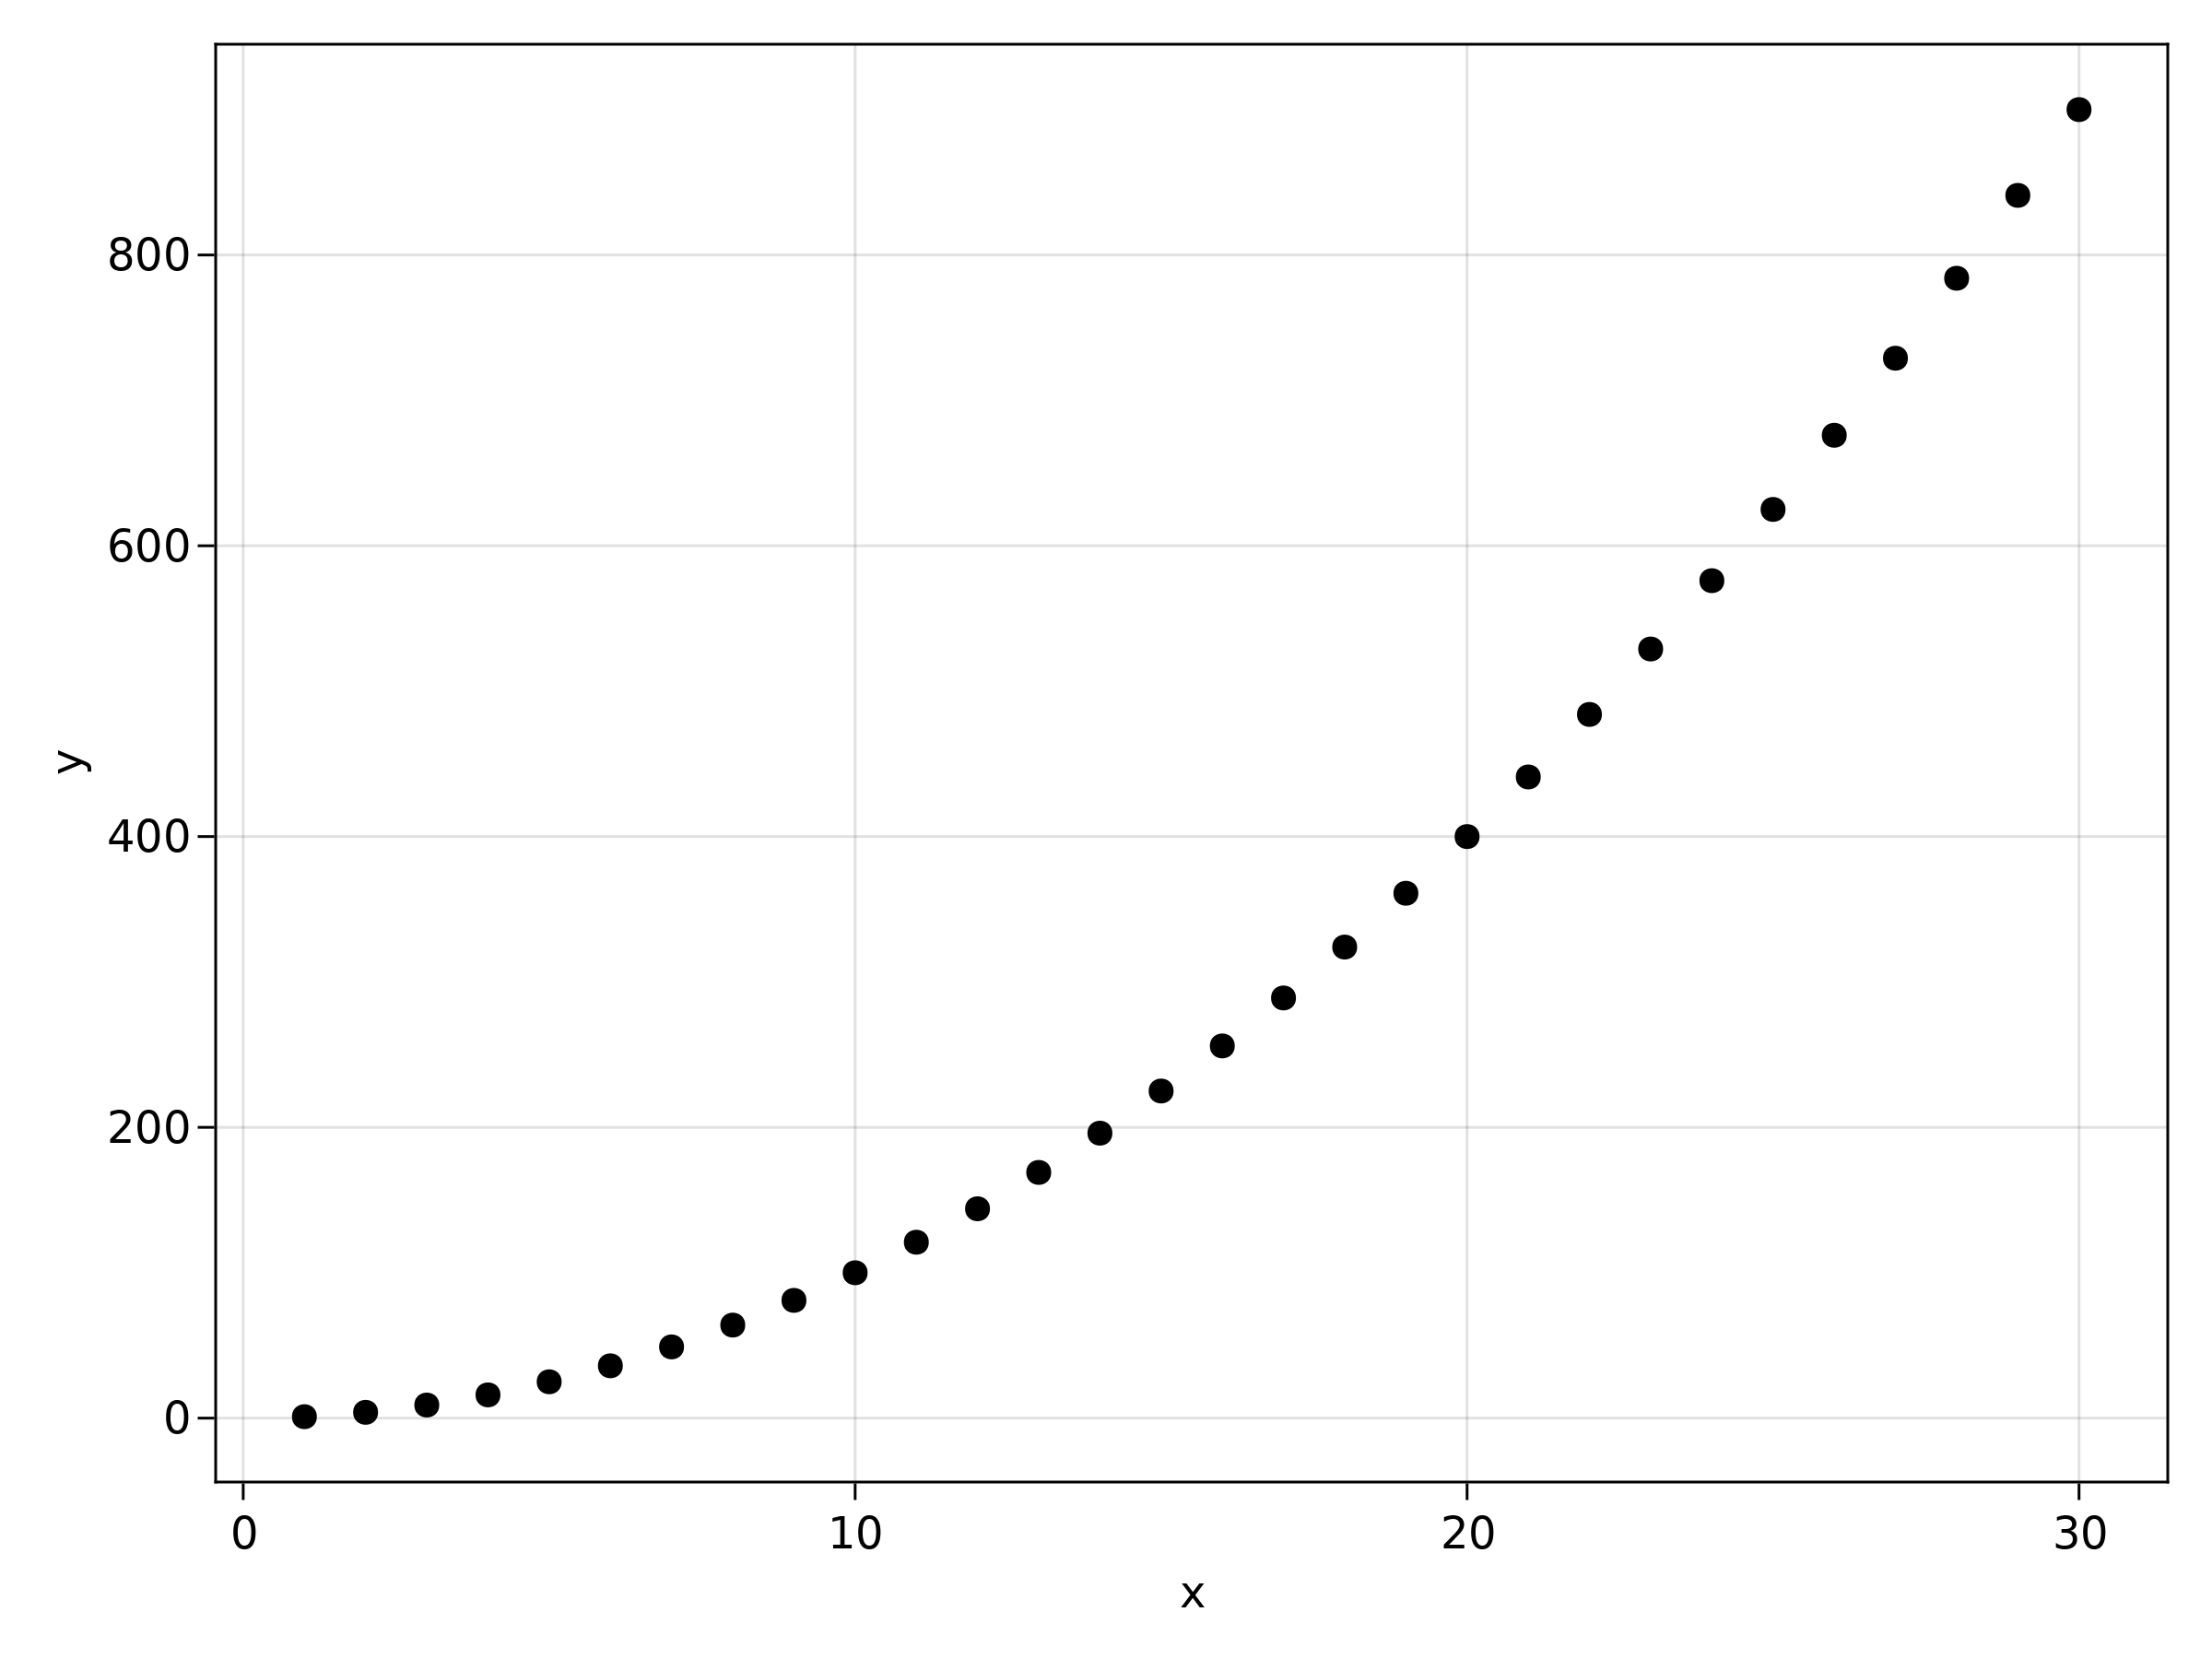
\includegraphics{_build/im/M_example_plot_.png}
\caption{Example plot.}\label{fig:example_plot}
}
\end{figure}

If the output is a string instead of the output you expected, then check
whether you load the related packages in time. For example, for this
plot, you need to load AlgebraOfGraphics.jl together with Books.jl so
that Requires.jl will load the code for handling AlgebraOfGraphics
objects.

For multiple images, use
\passthrough{\lstinline!Options.(objects, paths)!}:

\begin{lstlisting}
function multiple_example_plots()
    filenames = ["example_plot_$i" for i in 2:3]
    I = 1:30
    df = (x=I, y=I.*2, z=I.^3)
    objects = [
        draw(data(df) * mapping(:x, :y))
        draw(data(df) * mapping(:x, :z))
    ]
    Options.(objects, filenames)
end
\end{lstlisting}

Resulting in Figure~\ref{fig:example_plot_2} and
Figure~\ref{fig:example_plot_3}:

\begin{figure}
\hypertarget{fig:example_plot_2}{%
\centering
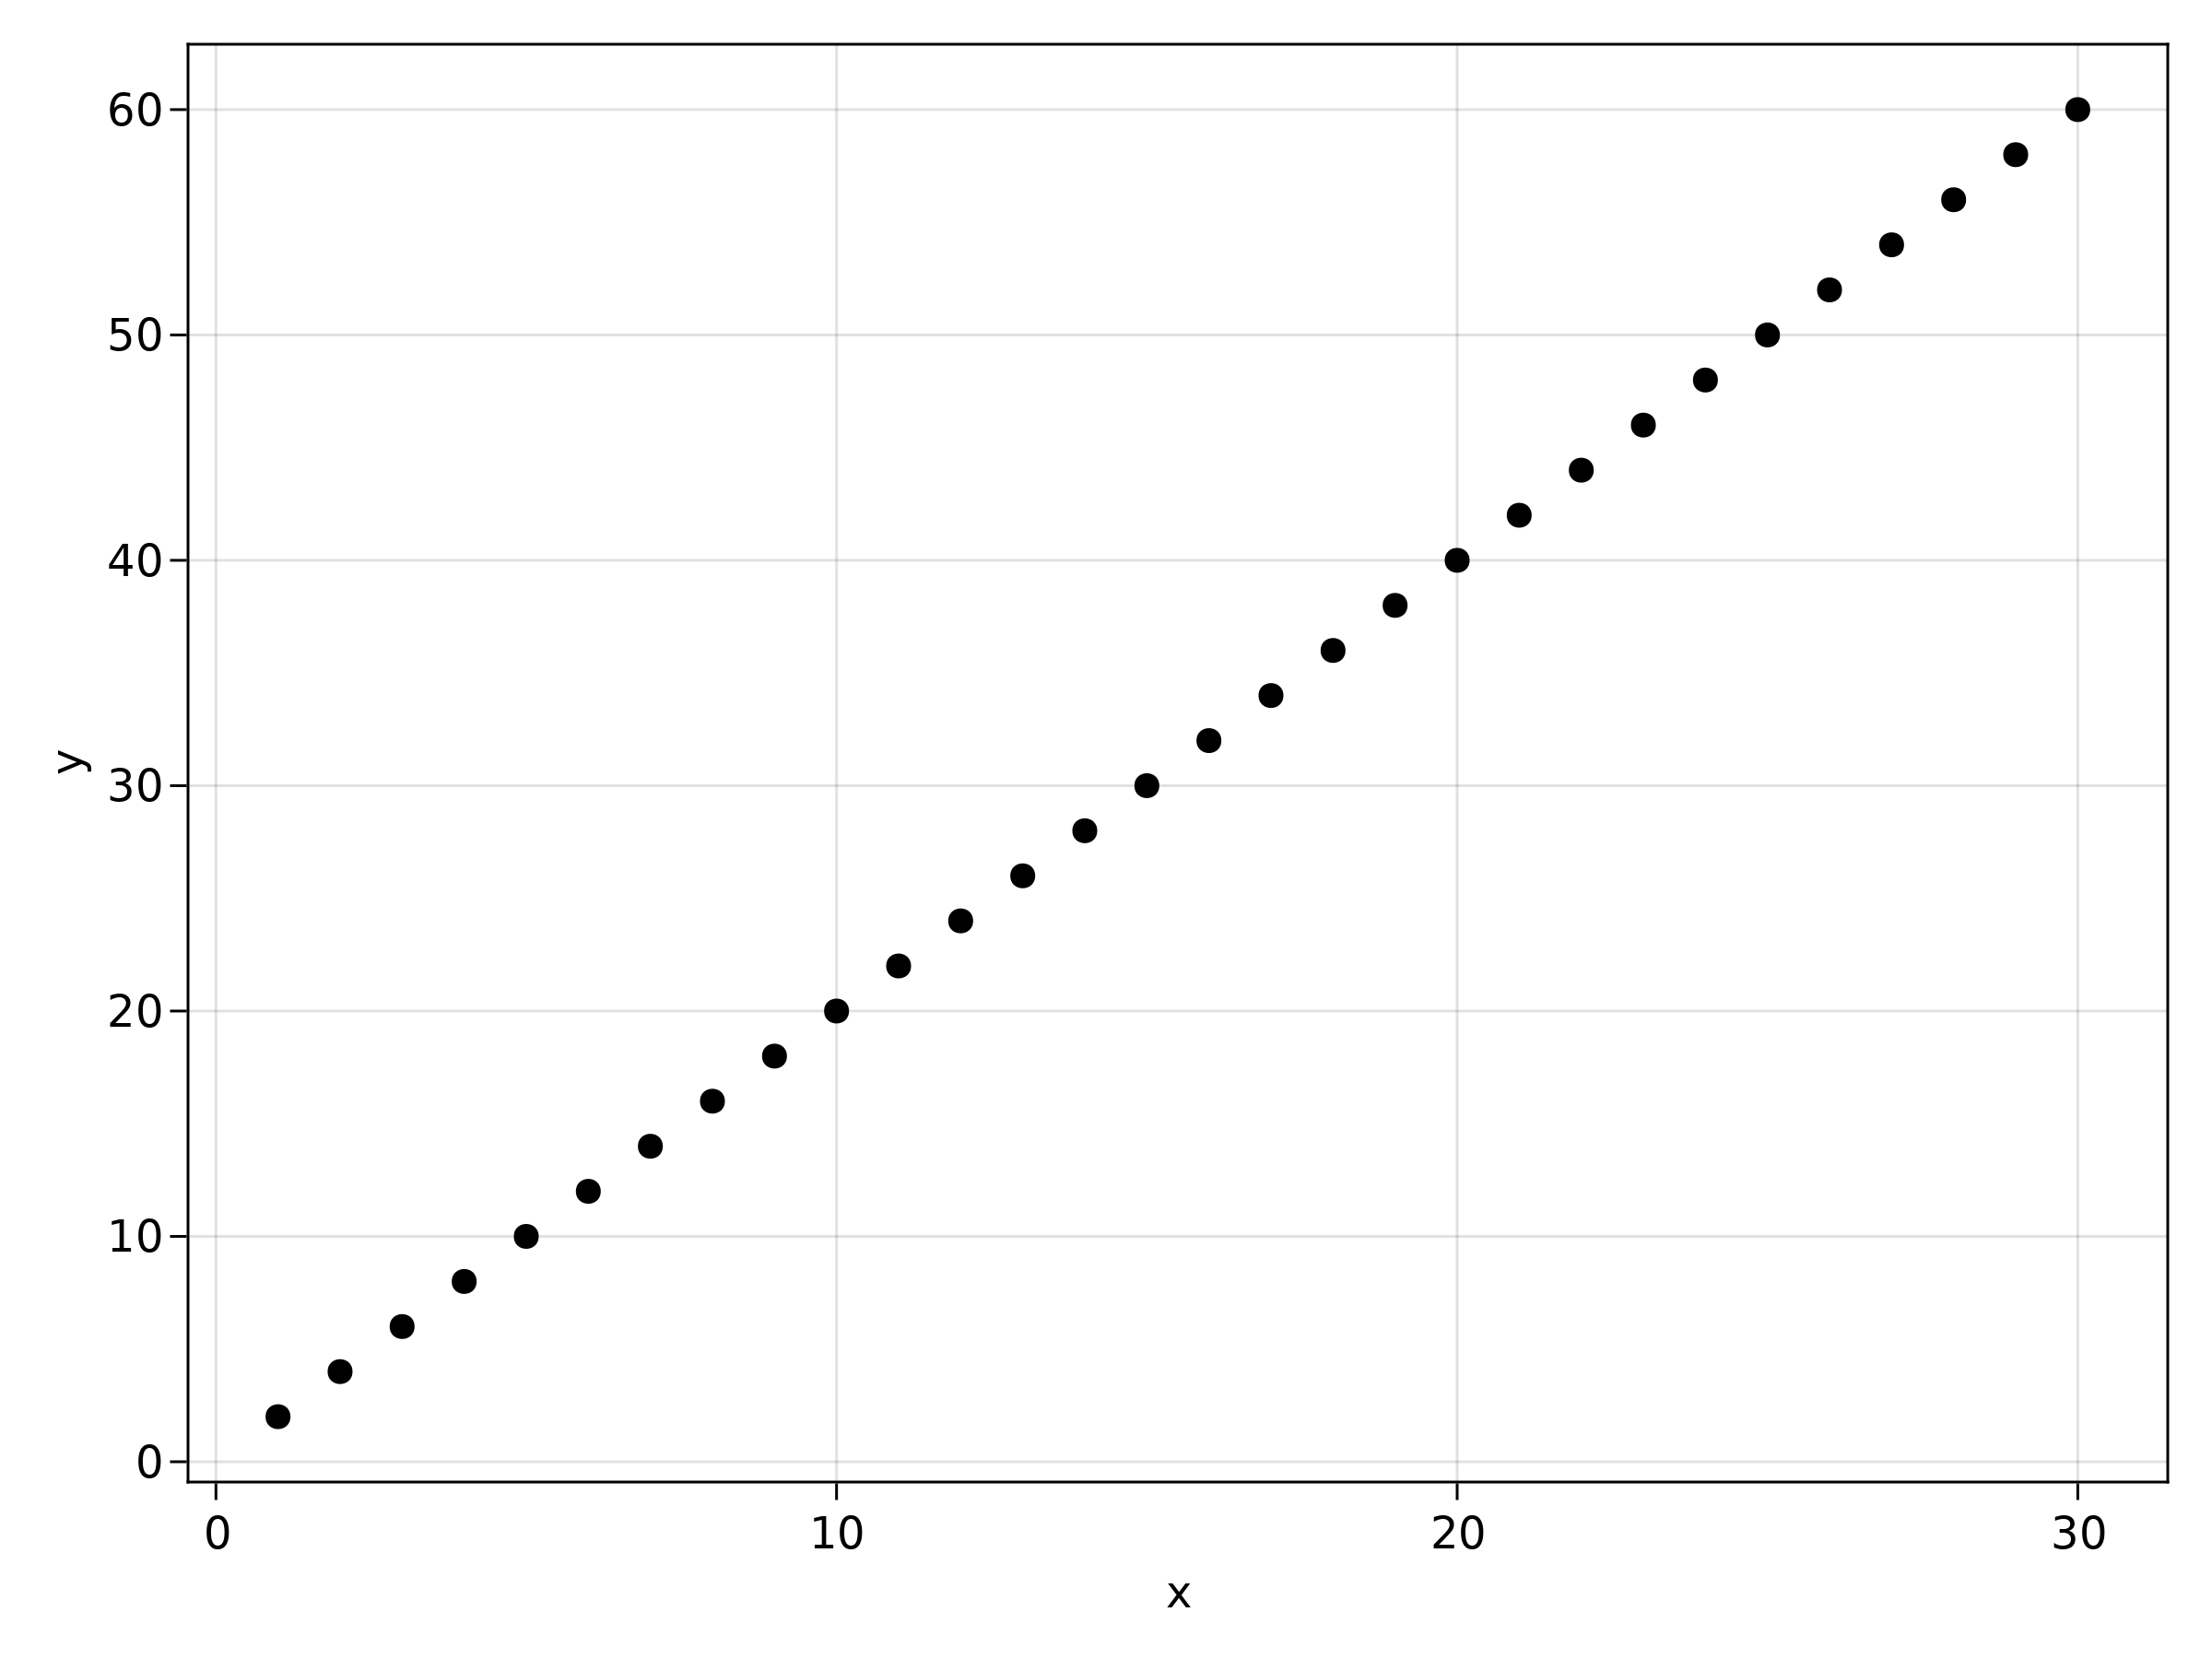
\includegraphics{_build/im/example_plot_2.png}
\caption{Example plot 2.}\label{fig:example_plot_2}
}
\end{figure}

\begin{figure}
\hypertarget{fig:example_plot_3}{%
\centering
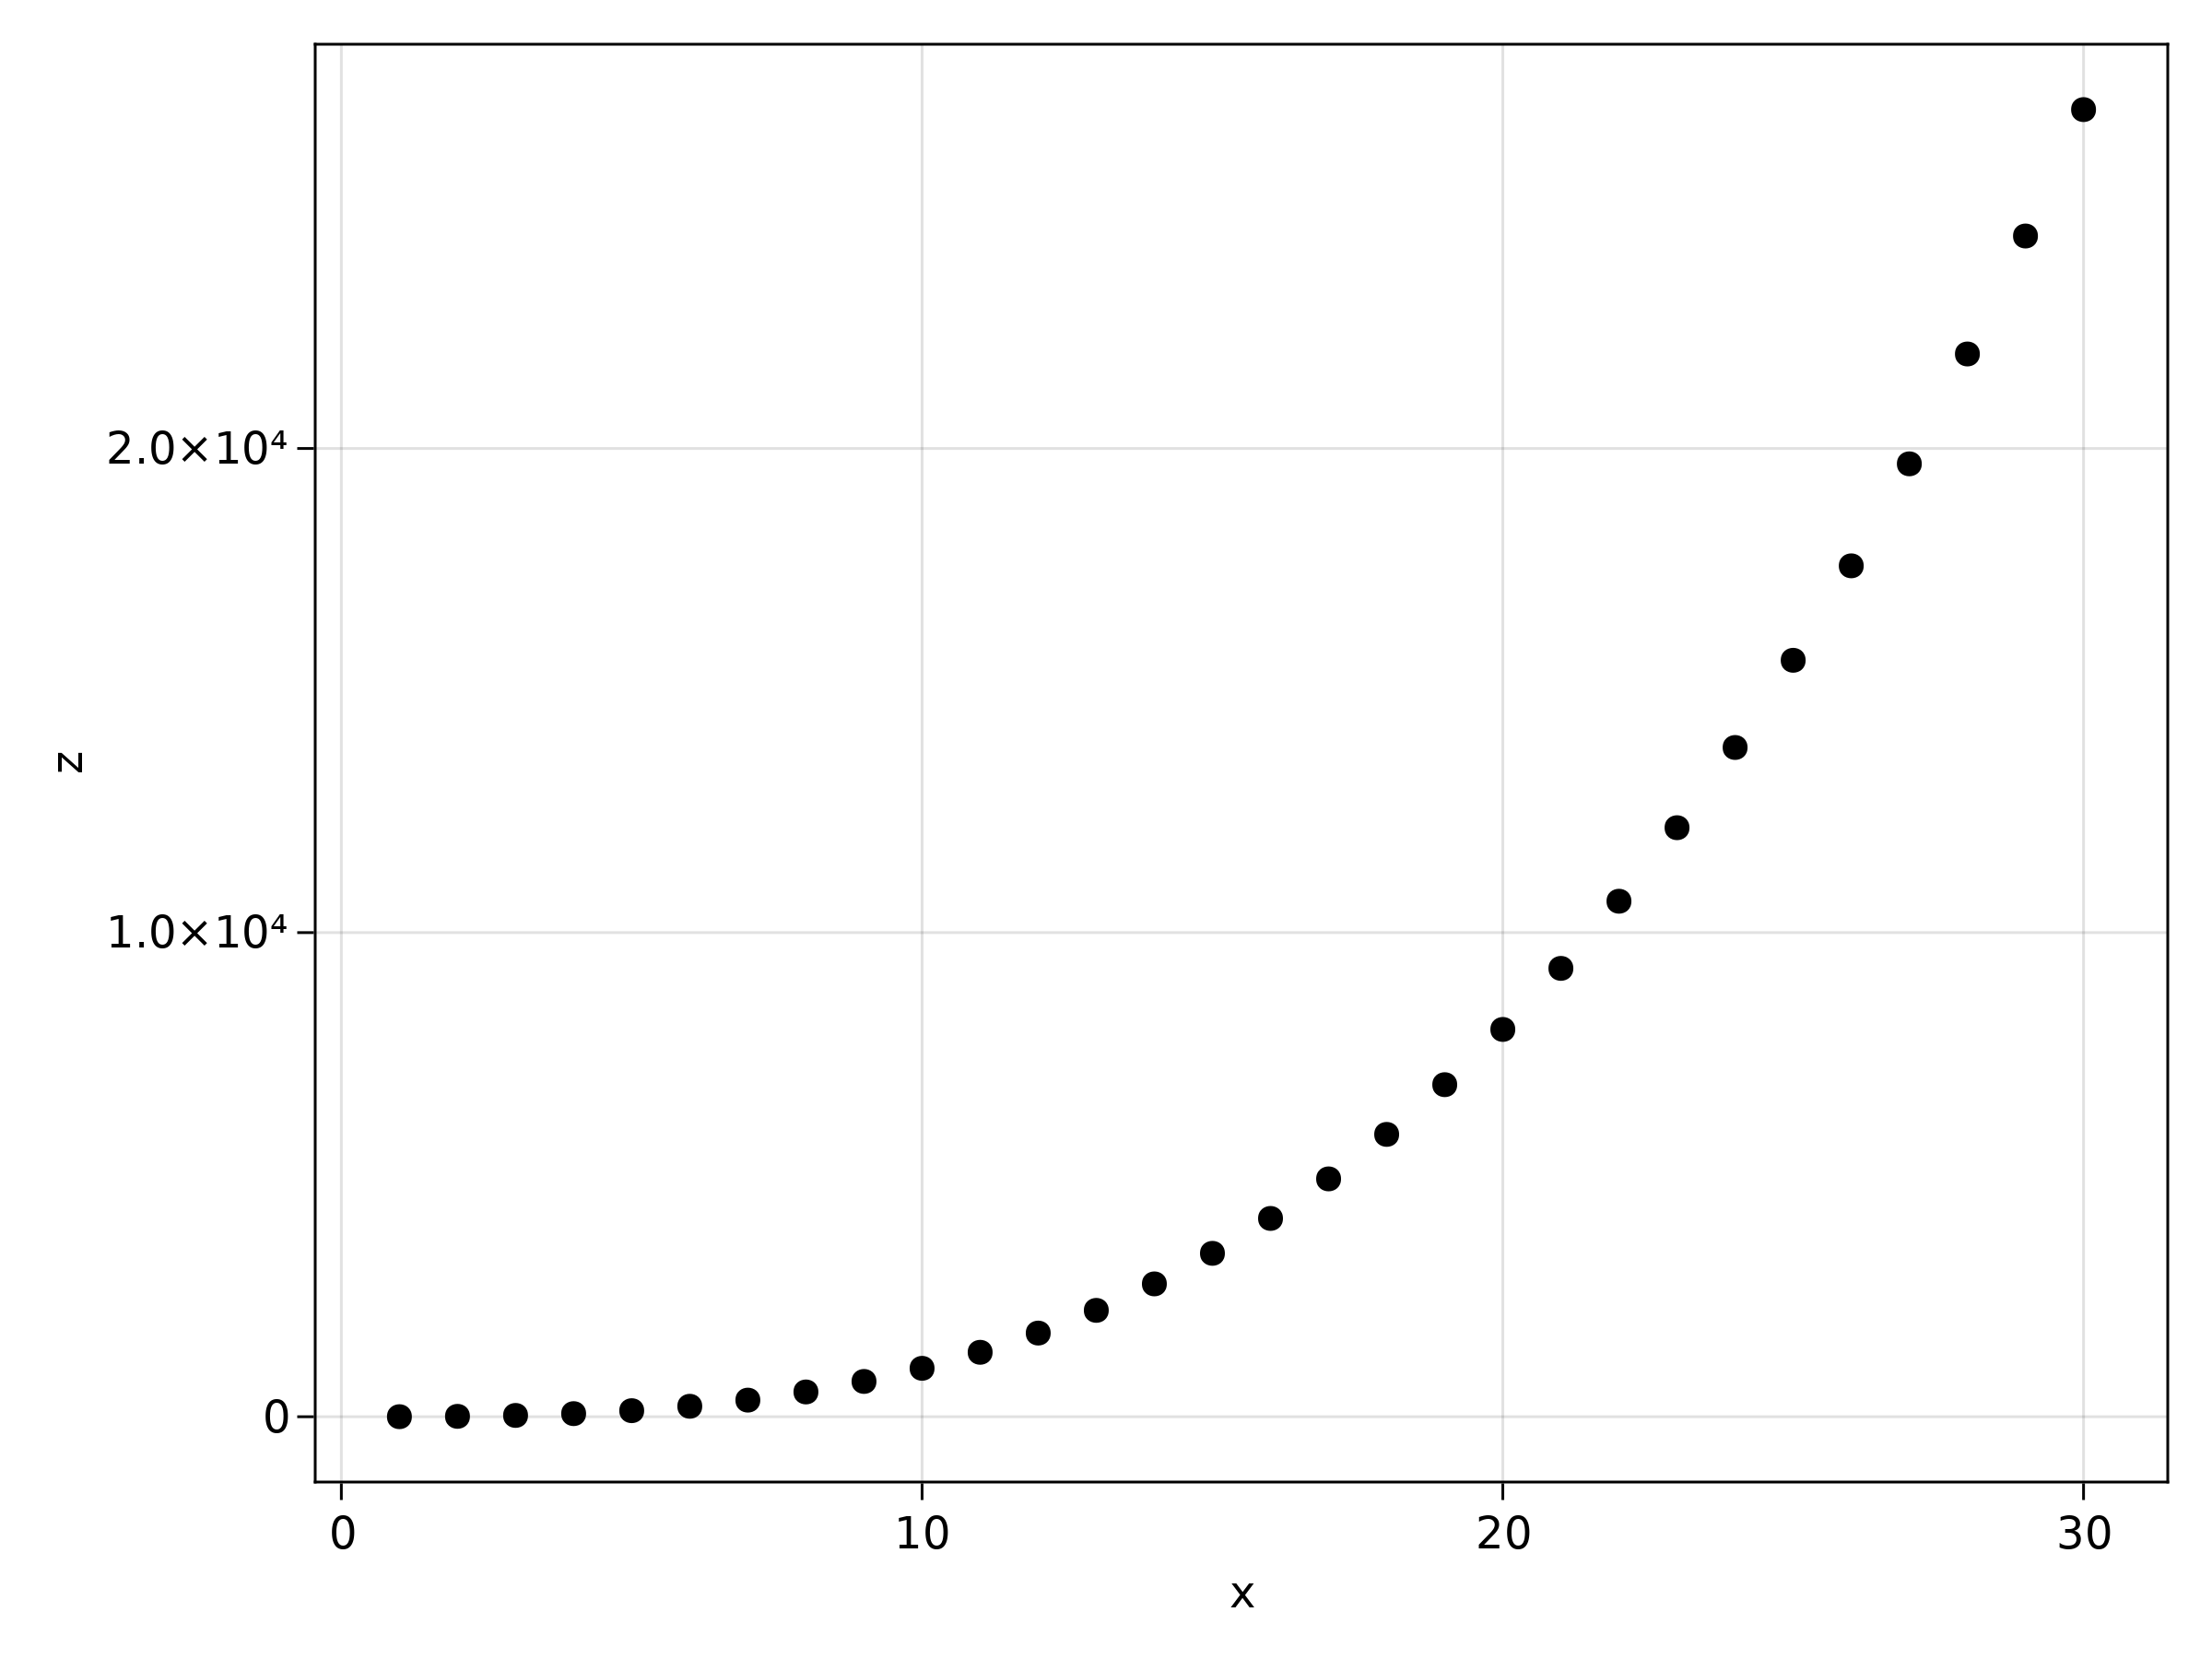
\includegraphics{_build/im/example_plot_3.png}
\caption{Example plot 3.}\label{fig:example_plot_3}
}
\end{figure}

For changing the size, use \passthrough{\lstinline!axis!} from
AlgebraOfGraphics:

\begin{lstlisting}
function image_options_plot()
    I = 1:0.1:30
    df = (x=I, y=sin.(I))
    xy = data(df) * visual(Lines) * mapping(:x, :y)
    axis = (width = 600, height = 140)
    draw(xy; axis)
end
image_options_plot()
\end{lstlisting}

\begin{figure}
\hypertarget{fig:image_options_plot}{%
\centering
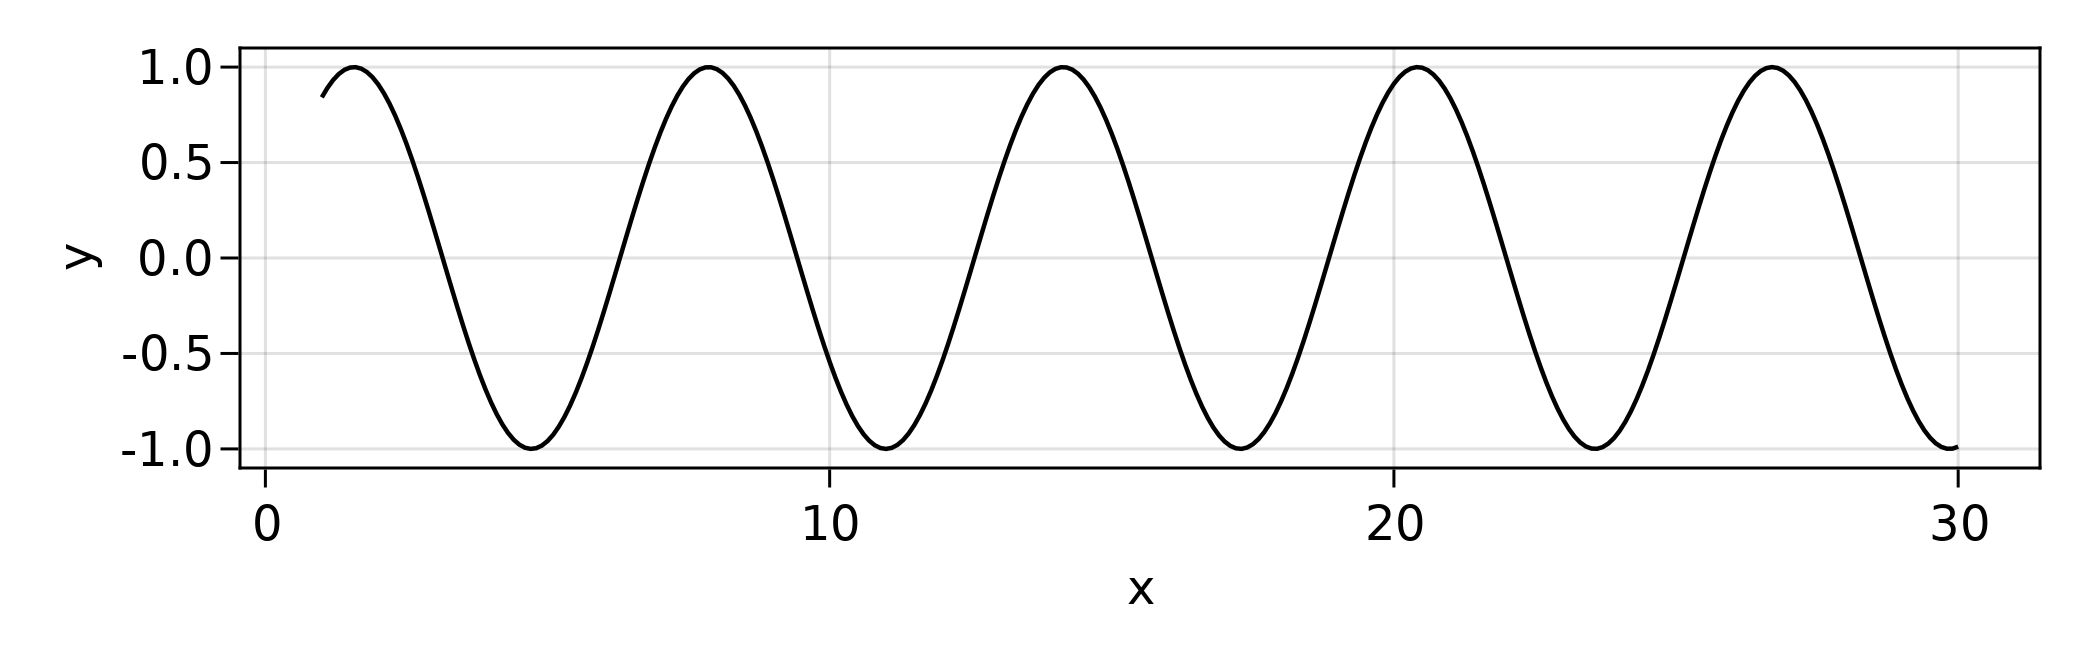
\includegraphics{_build/im/M_image_options_plot_.png}
\caption{Image options plot.}\label{fig:image_options_plot}
}
\end{figure}

And, for adjusting the caption, use \passthrough{\lstinline!Options!}:

\begin{lstlisting}
function combined_options_plot()
    fg = image_options_plot()
    Options(fg; caption="Sine function.")
end
combined_options_plot()
\end{lstlisting}

\begin{figure}
\centering
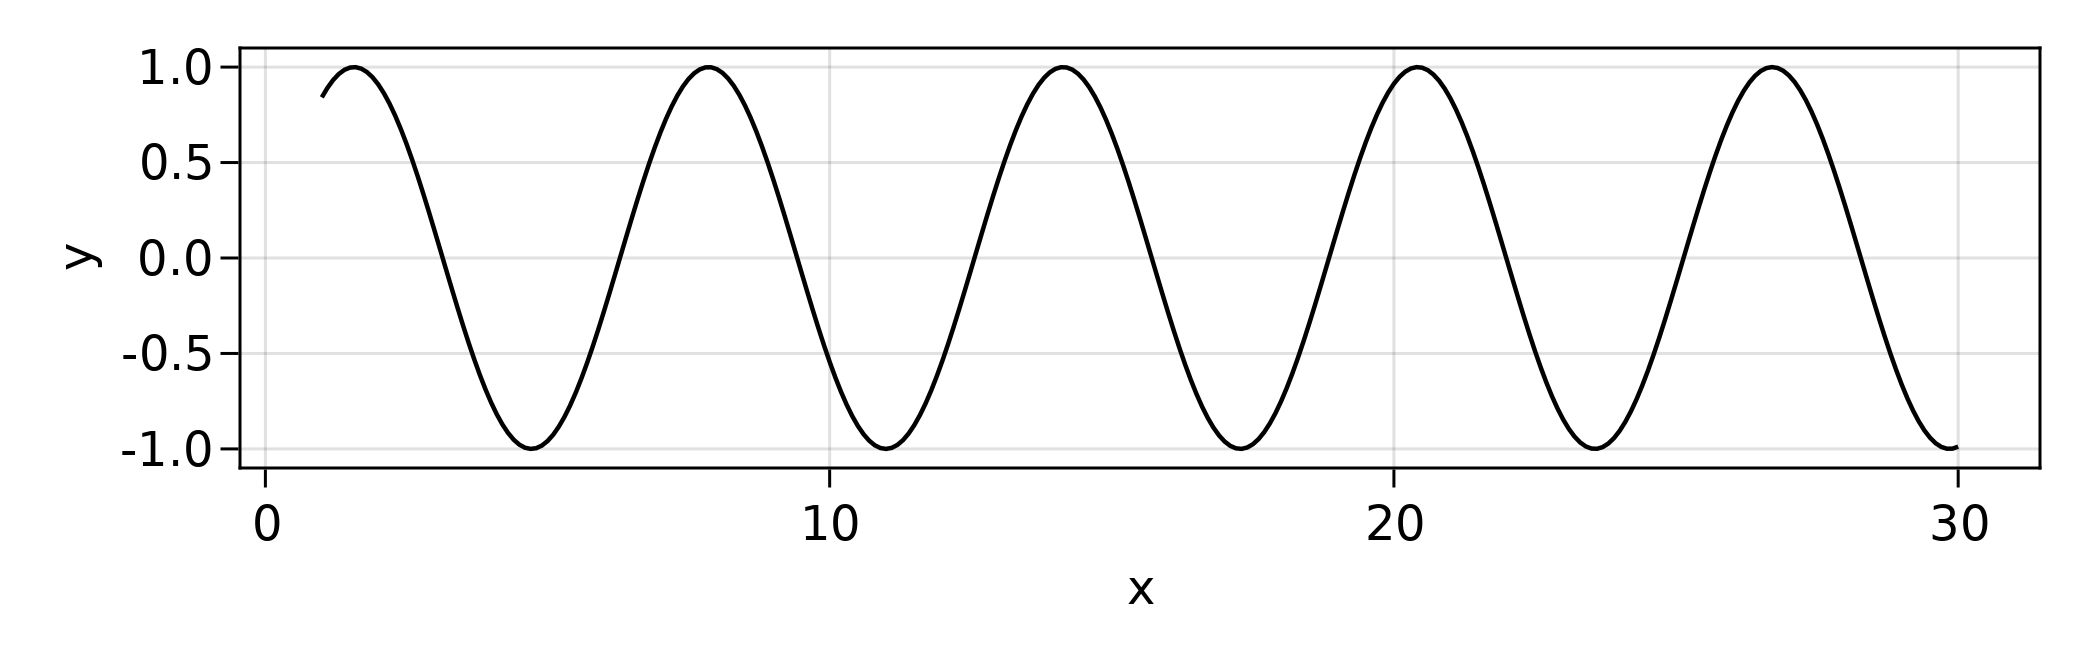
\includegraphics{_build/im/M_combined_options_plot_.png}
\caption{Sine function.}
\end{figure}

or the caption can be specified in the Markdown file:

\begin{figure}
\centering
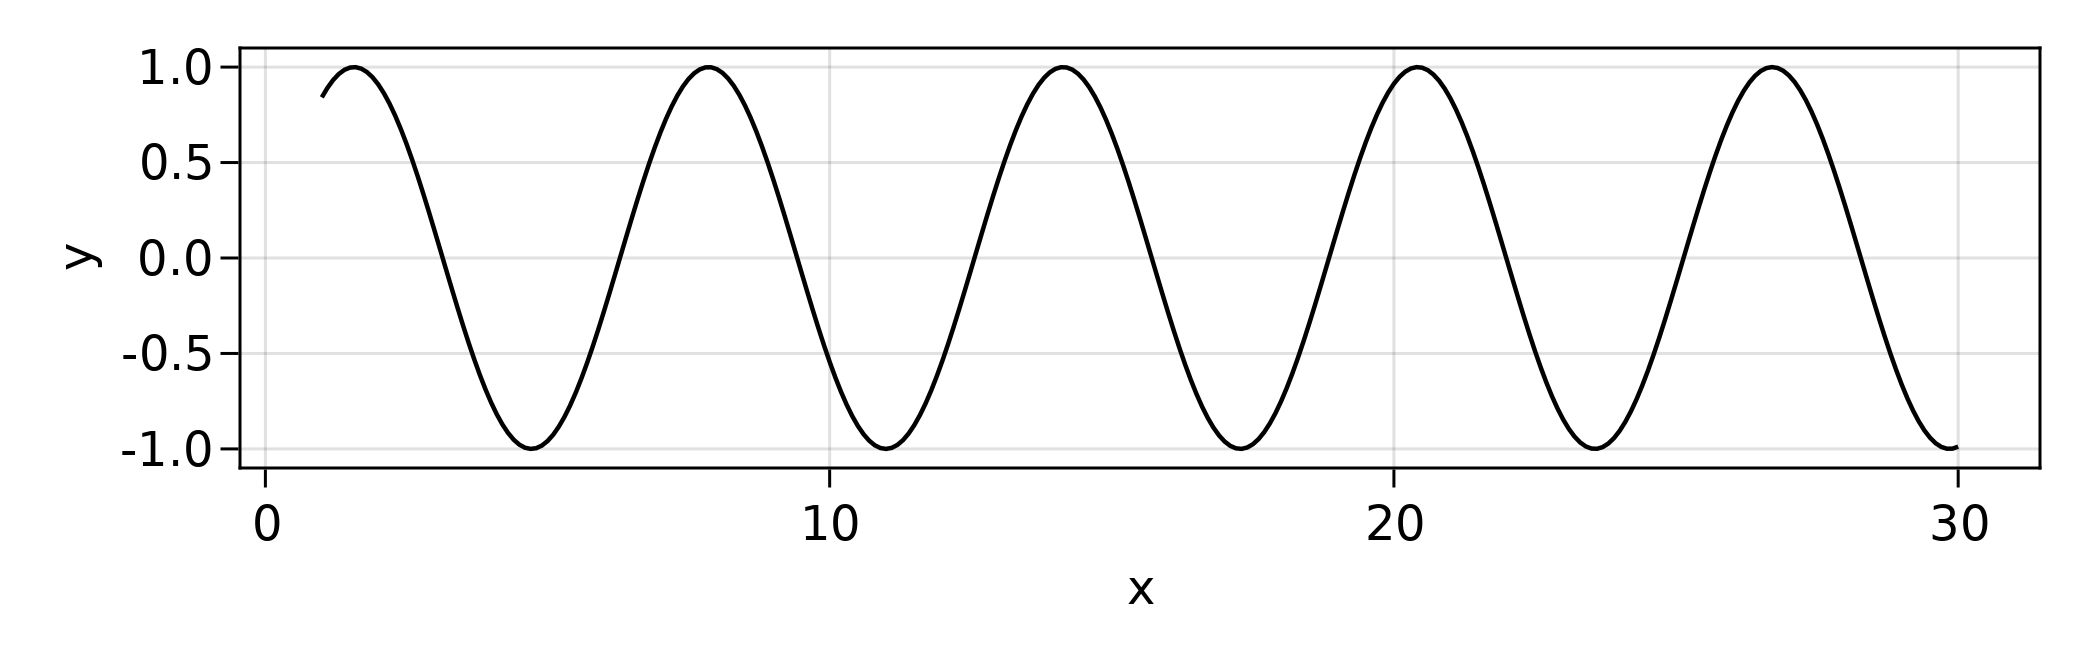
\includegraphics{_build/im/Options_M_image_options_plot_caption_Label_specified_in_Markdown_.png}
\caption{Label specified in Markdown.}
\end{figure}

\hypertarget{sec:plotsjl}{%
\subsection{Plots}\label{sec:plotsjl}}

\begin{lstlisting}
function plotsjl()
    p = plot(1:10, 1:2:20)
    caption = "An example plot with Plots.jl."
    # Label default to `nothing`, which will not create a cross-reference.
    label = missing
    Options(p; caption, label)
end
plotsjl()
\end{lstlisting}

\begin{figure}
\centering
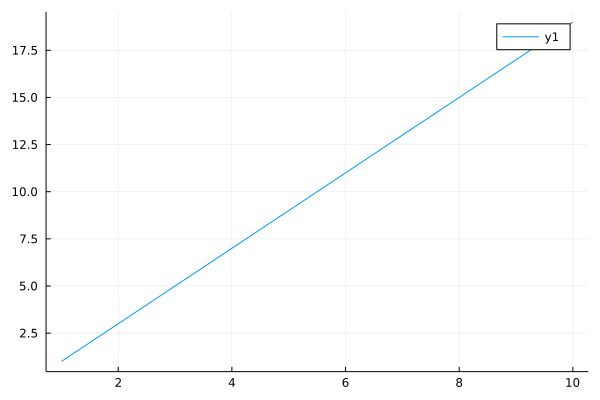
\includegraphics{_build/im/M_plotsjl_.png}
\caption{An example plot with Plots.jl.}
\end{figure}

\hypertarget{sec:makie}{%
\subsection{Makie}\label{sec:makie}}

\begin{lstlisting}
function makiejl()
    x = range(0, 10, length=100)
    y = sin.(x)
    p = lines(x, y)
    caption = "An example plot with Makie.jl."
    label = missing
    Options(p; caption, label)
end
makiejl()
\end{lstlisting}

\begin{figure}
\centering
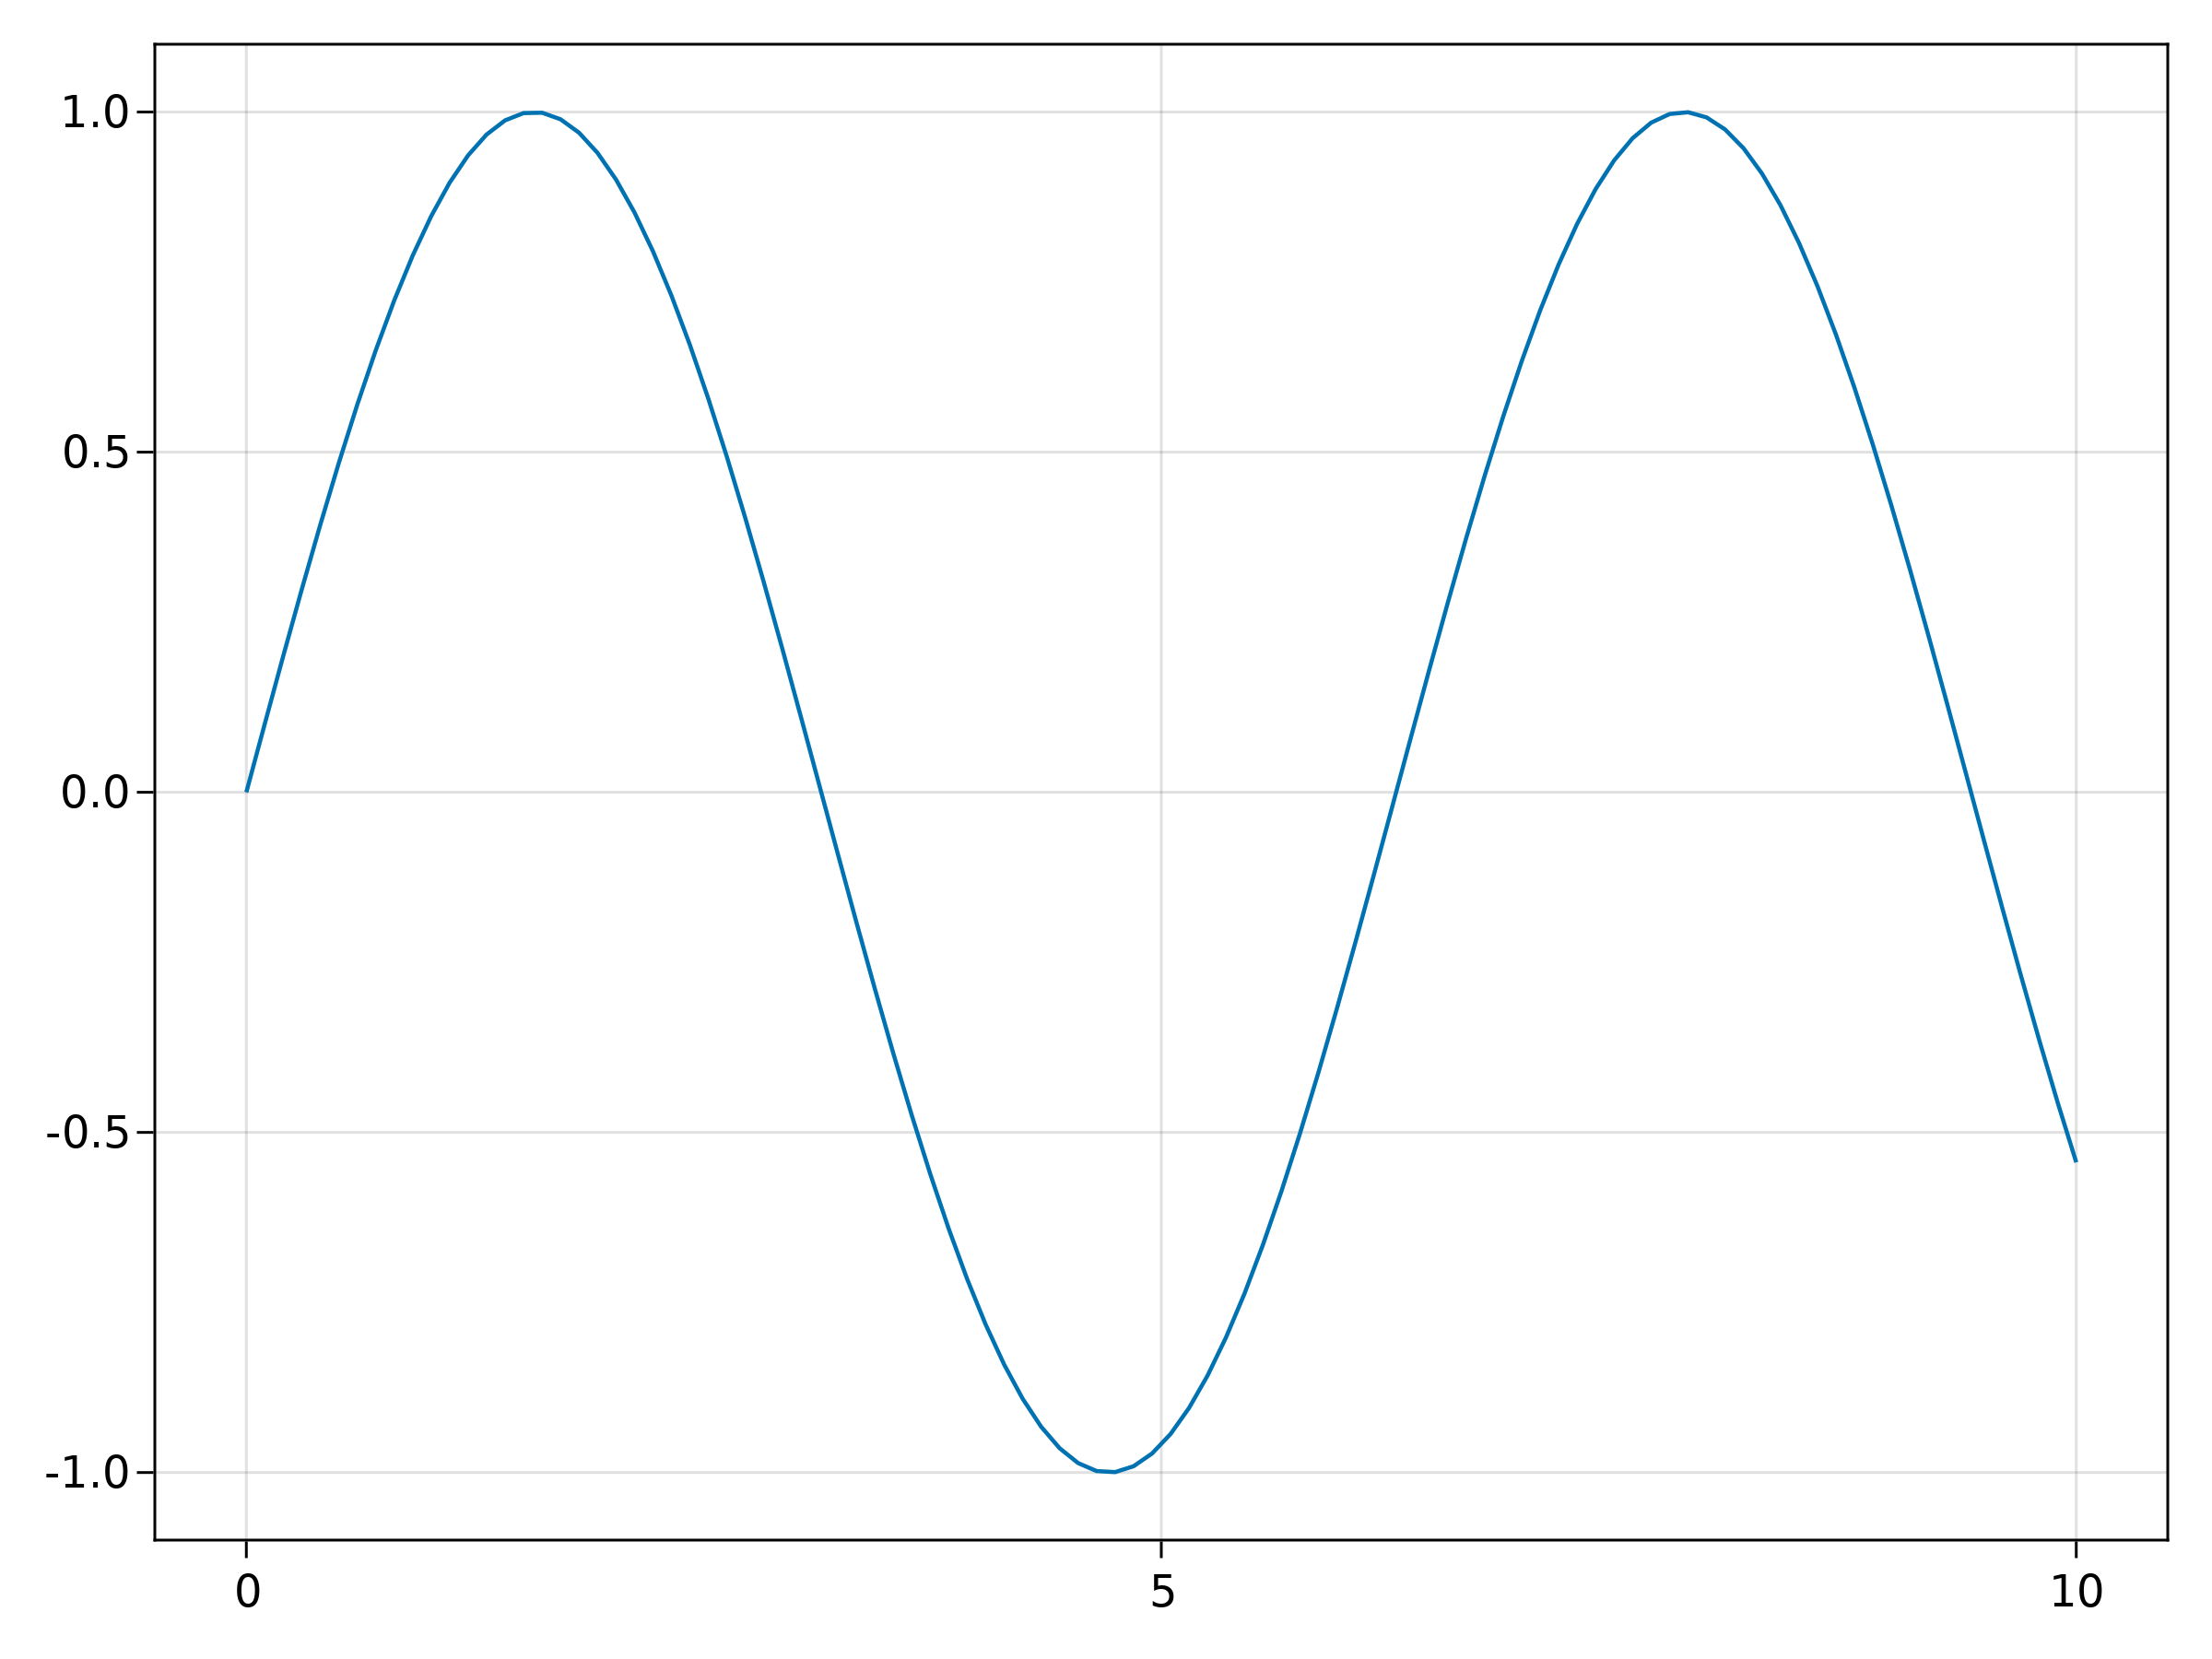
\includegraphics{_build/im/M_makiejl_.png}
\caption{An example plot with Makie.jl.}
\end{figure}

\hypertarget{other-notes}{%
\section{Other notes}\label{other-notes}}

\hypertarget{multilingual-books}{%
\subsection{Multilingual books}\label{multilingual-books}}

For an example of a multilingual book setup, say English and Chinese,
see the book by
\href{https://github.com/LearnJuliaTheFunWay/LearnJuliaTheFunWay.jl}{Jun
Tian}.

\hypertarget{show}{%
\subsection{Show}\label{show}}

When your method returns an output type \passthrough{\lstinline!T!}
which is unknown to Books.jl, it will be passed through
\passthrough{\lstinline!show(io::IO, ::MIME"text/plain", object::T)!}.
So, if the package that you're using has defined a new
\passthrough{\lstinline!show!} method, this will be used. For example,
for \passthrough{\lstinline!MCMCChains!},

\begin{lstlisting}
chain() = MCMCChains.Chains([1])
chain()
\end{lstlisting}

\begin{lstlisting}
Chains MCMC chain (1×1×1 Array{Int64, 3}):

Iterations        = 1:1:1
Number of chains  = 1
Samples per chain = 1
parameters        = param_1

Summary Statistics
  parameters      mean       std   naive_se      mcse       ess      rhat
      Symbol   Float64   Float64    Float64   Missing   Missing   Missing

     param_1    1.0000       NaN        NaN   missing   missing   missing

Quantiles
  parameters      2.5%     25.0%     50.0%     75.0%     97.5%
      Symbol   Float64   Float64   Float64   Float64   Float64

     param_1    1.0000    1.0000    1.0000    1.0000    1.0000
\end{lstlisting}

\hypertarget{note-box}{%
\subsection{Note box}\label{note-box}}

To write note boxes, you can use

\begin{lstlisting}
> **_NOTE:_**  The note content.
\end{lstlisting}

\begin{quote}
\textbf{\emph{NOTE:}} The note content.
\end{quote}

This way is fully supported by Pandoc, so it will be correctly converted
to outputs such as PDF or DOCX.

\hypertarget{advanced-sco-options}{%
\subsection{\texorpdfstring{Advanced \texttt{sco}
options}{Advanced sco options}}\label{advanced-sco-options}}

To enforce output to be embedded inside a code block, use
\passthrough{\lstinline!scob!}. For example,

\begin{lstlisting}
scob("
df = DataFrame(A = [1], B = [Date(2018)])
string(df)
")
\end{lstlisting}

\begin{lstlisting}
df = DataFrame(A = [1], B = [Date(2018)])
string(df)
\end{lstlisting}

\begin{lstlisting}
1×2 DataFrame
 Row │ A      B
     │ Int64  Date
─────┼───────────────────
   1 │     1  2018-01-01
\end{lstlisting}

or, with a string

\begin{lstlisting}
s = "Hello"
\end{lstlisting}

\begin{lstlisting}
Hello
\end{lstlisting}

Another way to change the output is via the keyword arguments
\passthrough{\lstinline!process!} and \passthrough{\lstinline!post!} for
\passthrough{\lstinline!sco!}.

which shows the following to the reader:

\begin{lstlisting}
df = DataFrame(A = [1], B = [Date(2018)])
\end{lstlisting}

\begin{lstlisting}
1×2 DataFrame
 Row │ A      B
     │ Int64  Date
─────┼───────────────────
   1 │     1  2018-01-01
\end{lstlisting}

Without \passthrough{\lstinline!process=string!}, the output would
automatically be converted to a Markdown table by Books.jl and then
wrapped inside a code block, which will cause Pandoc to show the raw
output instead of a table.

\begin{lstlisting}
df = DataFrame(A = [1], B = [Date(2018)])
\end{lstlisting}

\begin{lstlisting}
|   A |          B |
| ---:| ----------:|
|   1 | 2018-01-01 |
\end{lstlisting}

Without \passthrough{\lstinline!post=output\_block!}, the DataFrame
would be converted to a string, but not wrapped inside a code block so
that Pandoc will treat is as normal Markdown:

\begin{lstlisting}
df = DataFrame(A = [2], B = [Date(2018)])
\end{lstlisting}

Options(1×2 DataFrame Row │ A B │ Int64 Date ─────┼─────────────────── 1
│ 2 2018-01-01, missing, nothing, nothing)

This also works for \passthrough{\lstinline!@sco!}. For example, for
\passthrough{\lstinline!my\_data!} we can use:

which will show as:

\begin{lstlisting}
function my_data()
    DataFrame(A = [1, 2], B = [3, 4], C = [5, 6], D = [7, 8])
end
my_data()
\end{lstlisting}

\begin{lstlisting}
2×4 DataFrame
 Row │ A      B      C      D
     │ Int64  Int64  Int64  Int64
─────┼────────────────────────────
   1 │     1      3      5      7
   2 │     2      4      6      8
\end{lstlisting}

\hypertarget{fonts}{%
\subsection{Fonts}\label{fonts}}

The code blocks default to JuliaMono in html and PDF. Ligatures from
JuliaMono are disabled. For example, none of these symbols are combined
into a single glyph.

\begin{lstlisting}
|> => and <=
\end{lstlisting}

\hypertarget{long-lines-in-code-blocks}{%
\subsection{Long lines in code blocks}\label{long-lines-in-code-blocks}}

\begin{lstlisting}
When code or output is getting too long, a horizontal scrollbar is visible on the website to scroll horizontally.
\end{lstlisting}

\hypertarget{references}{%
\chapter*{References}\label{references}}
\addcontentsline{toc}{chapter}{References}

\hypertarget{refs}{}
\begin{CSLReferences}{1}{0}
\leavevmode\hypertarget{ref-orwell1945animal}{}%
Orwell, G. (1945). \emph{{Animal farm: a fairy story}}. Houghton Mifflin
Harcourt.

\leavevmode\hypertarget{ref-orwell1949nineteen}{}%
Orwell, G. (1949). \emph{{Nineteen eighty-four: a novel}}. Secker \&
Warburg.

\end{CSLReferences}

% \backmatter
\end{document}
